\chapter{Resultados computacionales}
\label{sec-results}
Los par\'ametros obtenidos en la secci\'on anterior~\ref{sec-validation} permiten ejecutar el aut\'omata celular concebido para la reproducci\'on del ciclo vital del c\'ancer. Los resultados que se presentan en esta secci\'on se obtuvieron promediando los datos provenientes de la ejecuci\'on de varias simulaciones del aut\'omata, preferiblemente un m\'inimo de $30$ simulaciones. En esta tarea se utiliz\'o un ordenador personal de gama baja-media con un procesador Intel Core $i3$ compuesto por $4$ n\'ucleos a una frecuencia de reloj de $2$.$2\,GHz$ y $8\,GB$ de memoria de acceso aleatorio ($RAM$). Se procede explorando en las secciones correspondientes~\ref{sec-avascular-results}--\ref{sec-metastasis-validation} los distintos comportamientos y etapas que presenta el c\'ancer, presentando los par\'ametros del modelo utilizados, la influencia de la variaci\'on de los mismos y las similitudes con los datos provenientes de otras investigaciones citadas respectivamente. En la secci\'on~\ref{subsec-scale-param} se expuso que la escala utilizada en la ejecuci\'on del aut\'omata es $1:3$. En cuanto a la asignaci\'on de los estados iniciales se utiliza el esquema I para el \'organo primario correspondiente con la mama, y el esquema III para el \'organo secundario correspondiente con los huesos como se mostr\'o en la secci\'on~\ref{subsec-states-param}, que en el caso del carcinoma ductal infiltrante constituye el destino m\'as frecuente de las met\'astasis. Partimos mostrando los par\'ametros de la construcci\'on de la red, de la asignaci\'on de estados iniciales y de las regiones y vectores de nutrientes en el cuadro~\ref{table-net-params}. 

\begin{table}[!ht]
\begin{center}
\scalebox{0.9}{\begin{tabular}{|p{2cm}|p{14.5cm}|}\hline
\emph{Red} & $s_x=1000$; $s_y=500$; $s_o=500$; $p = 0$.$01$. \\\hline

\emph{Estados} & Para el \'organo primario correspondiente con la mama -- Esquema I: $o_l=250$, $o_e=1$, $o_s=249$, $v_x^t=250$, $v_y^t=250$. Para el \'organo secundario correspondiente con los huesos -- Esquema III: $o_s=500$.\\\hline 

\emph{Nutrientes} & Para el \'organo primario -- $R_1 = \lbrace v~|~v \in V(G) : (0 \leq v_x < 500) \wedge (0 \leq v_y < 276) \rbrace$, $B_{01}=\lbrace \overrightarrow{\nu_{((0,0),(0,1))}} \rbrace$, $R_2 = \lbrace v~|~v \in V(G) : (0 \leq v_x < 500) \wedge (276 \leq v_y < 500) \rbrace$. Para el \'organo secundario -- $R_3 = \lbrace v~|~v \in V(G) : (500 \leq v_x < 1000) \wedge (0 \leq v_y < 500) \rbrace$.\\\hline
\end{tabular}}\vspace*{-0.5cm}
\end{center}
\caption[Valores de los par\'ametros de construcci\'on de la red, de la asignaci\'on de estados iniciales y de las regiones y vectores de nutrientes]{Valores de los par\'ametros de construcci\'on de la red, de la asignaci\'on de estados iniciales y de las regiones y vectores de nutrientes. Se utiliza la escala $1:3$ donde el tiempo transcurrido entre las generaciones del aut\'omata $n$ y $n+1$ se corresponde a $72$ horas y cada celda del aut\'omata contiene $9$ c\'elulas reales.}
\label{table-net-params}
\end{table}

\section{Crecimiento avascular}
\label{sec-avascular-results}
El primer conjunto de par\'ametros de la ley de crecimiento log\'istica, mostrada en las expresiones~(\ref{eq-pa}) y~(\ref{eq-pv}), describen el desarrollo de un tumor avascular de crecimiento r\'apido. Para ello se utilizan los valores de la poblaci\'on inicial y de las capacidades de carga m\'inimas, promedio y m\'aximas correspondientes con el intervalo de radios avasculares $R_a \in [0$.$5, 1]mm$ y una probabilidad m\'axima avascular $\rho_{max}^a=1$ como se muestran en el cuadro~\ref{table-avascular}. Los resultados provenientes de las simulaciones con los par\'ametros del cuadro~\ref{table-avascular} se muestran en las gr\'aficas~\ref{graph-avascular-simulations}. El an\'alisis de los resultados presentados se lleva a cabo en la secci\'on~\ref{sec-growth-validation}.
\begin{table}[!ht]
\begin{center}
\scalebox{0.9}{\begin{tabular}{|p{2.1cm}|p{14.5cm}|}\hline
\emph{M\'inimo} & $P_0^a=1$, $K_a=6$.$944 \times 10^1$, $r_a=5$.$797 \times 10^{-2}$, $\Delta t=1$.$693 \times 10^1$, $n_a=9$, generaciones del aut\'omata: $10$~($30$ d\'ias). \\\hline
\emph{Promedio} & $P_0^a=1$, $K_a=2$.$222 \times 10^2$, $r_a=1$.$802 \times 10^{-2}$, $\Delta t=2$.$996 \times 10^1$, $n_a=20$, generaciones del aut\'omata: $21$~($63$ d\'ias).\\\hline
\emph{M\'aximo} & $P_0^a=1$, $K_a=4$.$938 \times 10^2$, $r_a=8$.$097 \times 10^{-3}$, $\Delta t=4$.$558 \times 10^1$, $n_a=34$, generaciones del aut\'omata: $35$~($105$ d\'ias).\\\hline
\end{tabular}}\vspace*{-0.6cm}
\end{center}
\caption[Par\'ametros del desarrollo de un carcinoma ductal infiltrante de crecimiento r\'apido durante la etapa avascular]{Par\'ametros del desarrollo de un carcinoma ductal infiltrante de crecimiento r\'apido durante la etapa avascular.}
\label{table-avascular}
\end{table}

\begin{figure}[p]
\begin{center}
\subfigure[Crecimiento m\'inimo $K_a=6$.$944 \times 10^1$]{\scalebox{0.8}{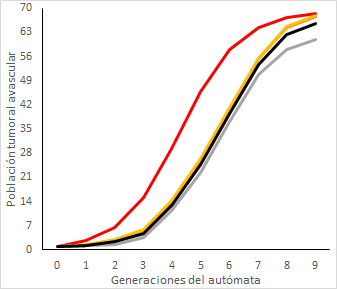
\includegraphics{img/graphs/graph-avascular-simulations-min.png}}
\scalebox{0.8}{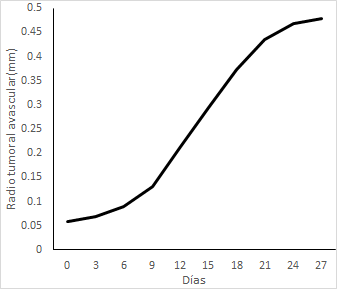
\includegraphics{img/graphs/graph-avascular-simulations-min-r.png}}}\vspace*{-0.2cm}
\subfigure[Crecimiento promedio $K_a=2$.$222 \times 10^2$]{\scalebox{0.8}{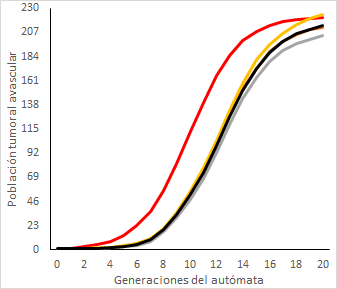
\includegraphics{img/graphs/graph-avascular-simulations-pro.png}}
\scalebox{0.8}{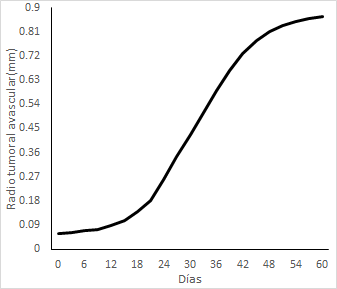
\includegraphics{img/graphs/graph-avascular-simulations-pro-r.png}}}\vspace*{-0.2cm}
\subfigure[Crecimiento m\'aximo $K_a=4$.$938 \times 10^2$]{\scalebox{0.8}{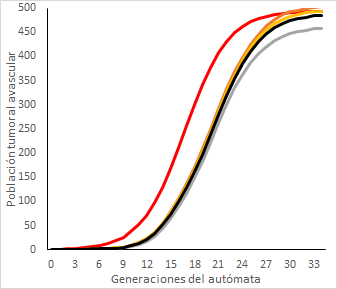
\includegraphics{img/graphs/graph-avascular-simulations-max.png}}
\scalebox{0.8}{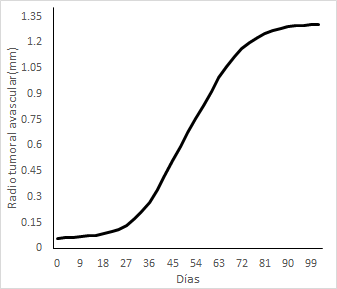
\includegraphics{img/graphs/graph-avascular-simulations-max-r.png}}}\vspace*{-0.2cm}
\end{center}\vspace*{-0.6cm}
\caption[Poblaci\'on y radios de un carcinoma ductal infiltrante de crecimiento r\'apido con $\rho_{max}^a=1$ durante la etapa avascular]{Poblaci\'on y radios de un carcinoma ductal infiltrante de crecimiento r\'apido con $\rho_{max}^a=1$ durante la etapa avascular. El resto de par\'ametros se muestran en el cuadro~\ref{table-avascular}. (a,b,c--izquierda) En rojo los valores obtenidos de la soluci\'on de la ley de crecimiento log\'istico, en negro los promedios de la poblaci\'on tumoral y el resto de curvas son varias simulaciones del aut\'omata. (a,b,c--derecha) En negro los promedios del radio tumoral.}
\label{graph-avascular-simulations}
\end{figure}

Con el objetivo de establecer comparaciones se determina un conjunto de par\'ametros del modelo de crecimiento log\'istico que describen el desarrollo de un tumor avascular de crecimiento lento. Para ello se utilizan los valores de la poblaci\'on inicial y de las capacidades de carga m\'inimas, promedio y m\'aximas correspondientes con el intervalo de radios avasculares $R_a \in [0$.$5, 1]mm$ y una probabilidad m\'axima avascular $\rho_{max}^a=0$.$1$ como se muestra en el cuadro~\ref{table-avascular-1}. El modelo puede reproducir tumores que toman mucho m\'as tiempo para su desarrollo pero se considera adecuado mostrar el crecimiento para la anterior probabilidad m\'axima $\rho_{max}^a=0$.$1$ para establecer dichas comparaciones; e.g. tumores con una probabilidad m\'axima menor como $\rho_{max}^a=0$.$01$. Los resultados provenientes de las simulaciones con los par\'ametros del cuadro~\ref{table-avascular-1} se muestran en las gr\'aficas~\ref{graph-avascular-simulations-1}. El an\'alisis de los resultados presentados se lleva a cabo en la secci\'on~\ref{sec-growth-validation}.
\begin{table}[!ht]
\begin{center}
\scalebox{0.9}{\begin{tabular}{|p{2.1cm}|p{14.5cm}|}\hline
\emph{M\'inimo} & $P_0^a=1$, $K_a=6$.$944 \times 10^1$, $r_a=5$.$797 \times 10^{-3}$, $\Delta t=2$.$854 \times 10^1$, $n_a=51$, generaciones del aut\'omata: $52$~($156$ d\'ias).\\\hline
\emph{Promedio} & $P_0^a=1$, $K_a=2$.$222 \times 10^2$, $r_a=1$.$802 \times 10^{-3}$, $\Delta t=5$.$497 \times 10^1$, $n_a=109$, generaciones del aut\'omata: $110$~($330$ d\'ias).\\\hline
\emph{M\'aximo} & $P_0^a=1$, $K_a=4$.$938 \times 10^2$, $r_a=8$.$097 \times 10^{-4}$, $\Delta t=8$.$604 \times 10^1$, $n_a=178$, generaciones del aut\'omata: $179$~($537$ d\'ias).\\\hline
\end{tabular}}\vspace*{-0.6cm}
\end{center}
\caption[Par\'ametros del desarrollo de un carcinoma ductal infiltrante de crecimiento lento durante la etapa avascular]{Par\'ametros del desarrollo de un carcinoma ductal infiltrante de crecimiento lento durante la etapa avascular.}
\label{table-avascular-1}
\end{table}

\begin{figure}[p]
\begin{center}
\subfigure[Crecimiento m\'inimo $K_a=6$.$944 \times 10^1$]{\scalebox{0.8}{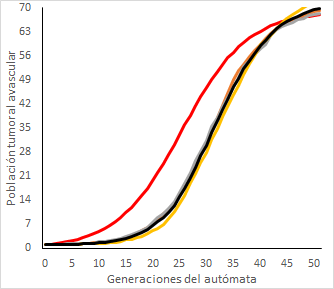
\includegraphics{img/graphs/graph-avascular-simulations-min-1.png}}
\scalebox{0.8}{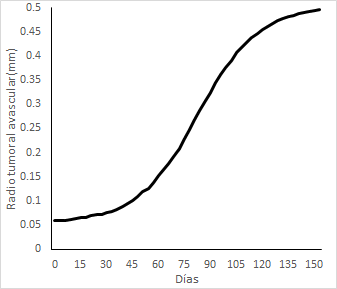
\includegraphics{img/graphs/graph-avascular-simulations-min-r-1.png}}}\vspace*{-0.2cm}
\subfigure[Crecimiento promedio $K_a=2$.$222 \times 10^2$]{\scalebox{0.8}{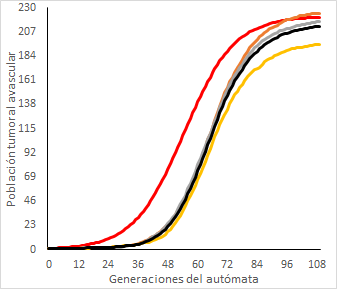
\includegraphics{img/graphs/graph-avascular-simulations-pro-1.png}}
\scalebox{0.8}{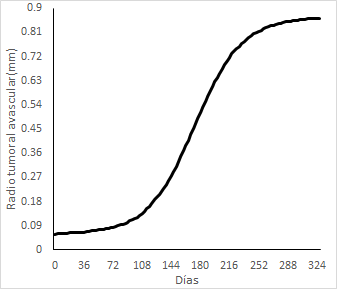
\includegraphics{img/graphs/graph-avascular-simulations-pro-r-1.png}}}\vspace*{-0.2cm}
\subfigure[Crecimiento m\'aximo $K_a=4$.$938 \times 10^2$]{\scalebox{0.8}{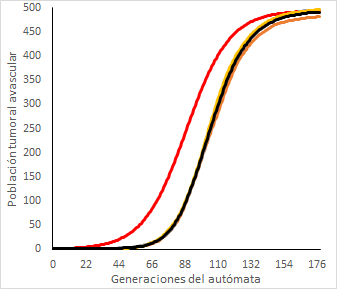
\includegraphics{img/graphs/graph-avascular-simulations-max-1.png}}
\scalebox{0.8}{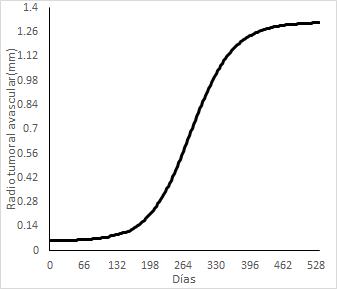
\includegraphics{img/graphs/graph-avascular-simulations-max-r-1.png}}}\vspace*{-0.2cm}
\end{center}\vspace*{-0.6cm}
\caption[Poblaci\'on y radios de un carcinoma ductal infiltrante de crecimiento lento con $\rho_{max}^a=0$.$1$ durante la etapa avascular]{Poblaci\'on y radios de un carcinoma ductal infiltrante de crecimiento lento con $\rho_{max}^a=0$.$1$ durante la etapa avascular. El resto de par\'ametros se muestran en el cuadro~\ref{table-avascular-1}. (a,b,c--izquierda) En rojo los valores obtenidos de la soluci\'on de la ley de crecimiento log\'istico, en negro los promedios de la poblaci\'on tumoral y el resto de curvas son varias simulaciones del aut\'omata. (a,b,c--derecha) En negro los promedios del radio tumoral.}
\label{graph-avascular-simulations-1}
\end{figure}

En la figura~\ref{fig-avascular-automata} se muestran las visualizaciones de una de las simulaciones del aut\'omata de un carcinoma ductal infiltrante de crecimiento r\'apido durante la etapa avascular. Al tratarse de un carcinoma que constituye un tipo de c\'ancer que surge en el epitelio~(en naranja) se puede apreciar que comienza su desarrollo en esta capa de tejido. Se puede apreciar, adem\'as, la adecuada aplicaci\'on de la regla del crecimiento tumoral definida en la secci\'on~\ref{subsec-celldiv} que establece que durante la etapa avascular un tumor primario no puede penetrar la membrana basal e invadir el estroma~(en gris). En ninguna de las im\'agenes se evidencia esta invasi\'on. La influencia de los vectores de concentraci\'on de nutrientes definen la direcci\'on de la expansi\'on tumoral~(en negro) que se mantiene paralela al epitelio y avanza de forma limitada hacia el lumen~(en blanco). La invasi\'on del estroma tiene lugar durante la etapa vascular del tumor primario y durante las etapas avascular y vascular en tumores secundarios. 
\begin{figure}[!ht]
\begin{center}
\subfigure[Generaci\'on 0]{\scalebox{0.29}{
\includegraphics{img/automata/2019519191641-0.png}}}
\subfigure[Generaci\'on 4]{\scalebox{0.29}{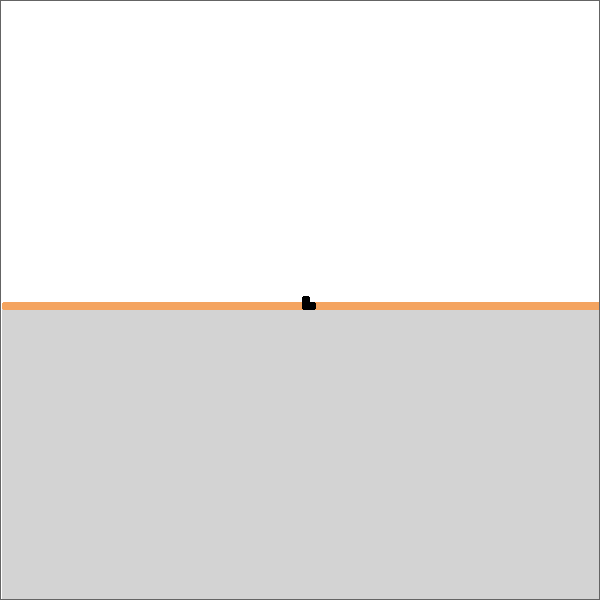
\includegraphics{img/automata/2019519191641-4.png}}}
\subfigure[Generaci\'on 8]{\scalebox{0.29}{
\includegraphics{img/automata/2019519191641-8.png}}}\vspace*{-0.25cm}
\subfigure[Generaci\'on 12]{\scalebox{0.29}{
\includegraphics{img/automata/2019519191641-12.png}}}
\subfigure[Generaci\'on 16]{\scalebox{0.29}{
\includegraphics{img/automata/2019519191641-16.png}}}
\subfigure[Generaci\'on 20]{\scalebox{0.29}{
\includegraphics{img/automata/2019519191641-20.png}}}\vspace*{-0.25cm}
\end{center}\vspace*{-0.6cm}
\caption[Visualizaciones de una simulaci\'on del aut\'omata celular de un carcinoma ductal infiltrante de crecimiento r\'apido durante la etapa avascular]{Visualizaciones de una simulaci\'on del aut\'omata celular de un carcinoma ductal infiltrante de crecimiento r\'apido durante la etapa avascular. Las generaciones del aut\'omata mostradas se obtienen mediante los par\'ametros correspondientes con la capacidad de carga promedio~(cuadro~\ref{table-avascular}). El \'area mostrada posee dimensiones $[0,10$.$5]mm \times [0,10$.$5]mm$.}
\label{fig-avascular-automata}
\end{figure}

\section{Crecimiento vascular}
\label{sec-vascular-results}
Este conjunto de par\'ametros de la ley de crecimiento log\'istica describen el desarrollo de un tumor vascular de crecimiento r\'apido. Para ello se utilizan los valores de la poblaci\'on inicial y de las capacidades de carga m\'inimas, promedio y m\'aximas correspondientes con el intervalo de radios vasculares $R_v \in [10, 15]mm$ y una probabilidad m\'axima vascular $\rho_{max}^v=1$ como se muestra en el cuadro~\ref{table-vascular}. La poblaci\'on inicial utilizada es la capacidad de carga avascular promedio, es decir, $P_0^v = K_a = 2$.$222 \times 10^2$. Los resultados provenientes de las simulaciones con los par\'ametros del cuadro~\ref{table-vascular} se muestran en las gr\'aficas~\ref{graph-vascular-simulations}. El an\'alisis de los resultados presentados se lleva a cabo en la secci\'on~\ref{sec-growth-validation}.
\begin{table}[!ht]
\begin{center}
\scalebox{0.9}{\begin{tabular}{|p{2.1cm}|p{14.5cm}|}\hline
\emph{M\'inimo} & $P_0^v=2$.$222 \times 10^2$, $K_v=2$.$778 \times 10^4$, $r_v=1$.$44 \times 10^{-4}$, $\Delta t=5$.$401 \times 10^2$, generaciones del aut\'omata: $121$~($363$ d\'ias).\\\hline
\emph{Promedio} & $P_0^v=2$.$222 \times 10^2$, $K_v=5$.$556 \times 10^4$, $r_v=7$.$199 \times 10^{-5}$, $\Delta t=7$.$665 \times 10^2$, generaciones del aut\'omata: $201$~($603$ d\'ias).\\\hline
\emph{M\'aximo} & $P_0^v=2$.$222 \times 10^2$, $K_v=1$.$111 \times 10^5$, $r_v=3$.$6 \times 10^{-5}$, $\Delta t=1$.$079 \times 10^3$, generaciones del aut\'omata: $321$~($963$ d\'ias).\\\hline
\end{tabular}}\vspace*{-0.6cm}
\end{center}
\caption[Par\'ametros del desarrollo de un carcinoma ductal infiltrante de crecimiento r\'apido durante la etapa vascular]{Par\'ametros del desarrollo de un carcinoma ductal infiltrante de crecimiento r\'apido durante la etapa vascular.}
\label{table-vascular}
\end{table}

\begin{figure}[p]
\begin{center}
\subfigure[Crecimiento m\'inimo $K_v=2$.$778 \times 10^4$]{\scalebox{0.8}{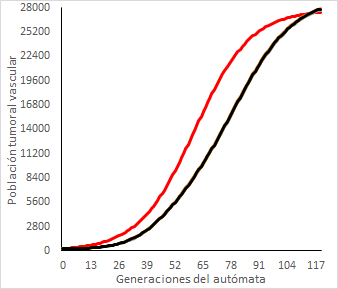
\includegraphics{img/graphs/graph-vascular-simulations-min.png}}
\scalebox{0.8}{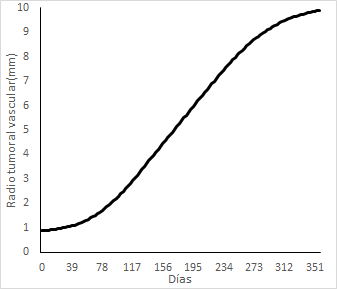
\includegraphics{img/graphs/graph-vascular-simulations-min-r.png}}}\vspace*{-0.2cm}
\subfigure[Crecimiento promedio $K_v=5$.$556 \times 10^4$]{\scalebox{0.8}{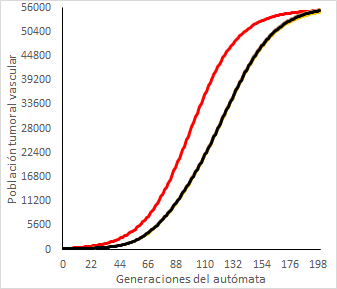
\includegraphics{img/graphs/graph-vascular-simulations-pro.png}}
\scalebox{0.8}{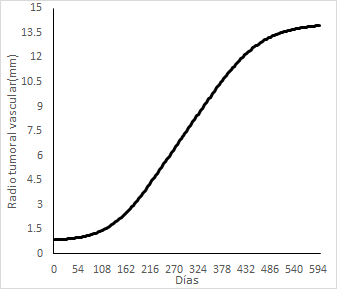
\includegraphics{img/graphs/graph-vascular-simulations-pro-r.png}}}\vspace*{-0.2cm}
\subfigure[Crecimiento m\'aximo $K_v=1$.$111 \times 10^5$]{\scalebox{0.8}{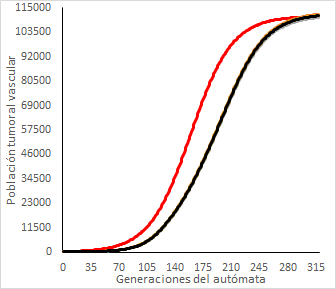
\includegraphics{img/graphs/graph-vascular-simulations-max.png}}
\scalebox{0.8}{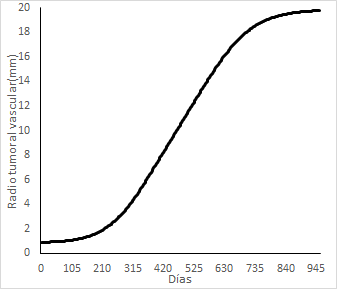
\includegraphics{img/graphs/graph-vascular-simulations-max-r.png}}}\vspace*{-0.2cm}
\end{center}\vspace*{-0.6cm}
\caption[Poblaci\'on y radios de un carcinoma ductal infiltrante de crecimiento r\'apido con $\rho_{max}^v=1$ durante la etapa vascular]{Poblaci\'on y radios de un carcinoma ductal infiltrante de crecimiento r\'apido con $\rho_{max}^v=1$ durante la etapa vascular. El resto de par\'ametros se muestran en el cuadro~\ref{table-vascular}. (a,b,c--izquierda) En rojo los valores obtenidos de la soluci\'on de la ley de crecimiento log\'istico, en negro los promedios de la poblaci\'on tumoral y el resto de curvas son varias simulaciones del aut\'omata. (a,b,c--derecha) En negro los promedios del radio tumoral.}
\label{graph-vascular-simulations}
\end{figure}

\begin{figure}[p]
\begin{center}
\subfigure[Crecimiento m\'inimo $K_v=2$.$778 \times 10^4$]{\scalebox{0.8}{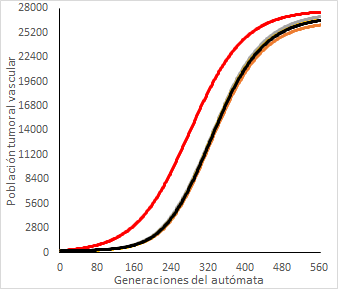
\includegraphics{img/graphs/graph-vascular-simulations-min-1.png}}
\scalebox{0.8}{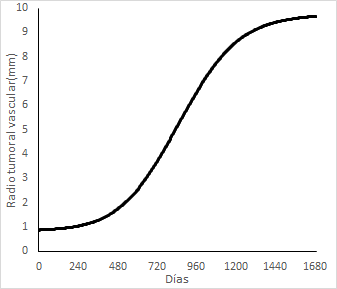
\includegraphics{img/graphs/graph-vascular-simulations-min-r-1.png}}}\vspace*{-0.2cm}
\subfigure[Crecimiento promedio $K_v=5$.$556 \times 10^4$]{\scalebox{0.8}{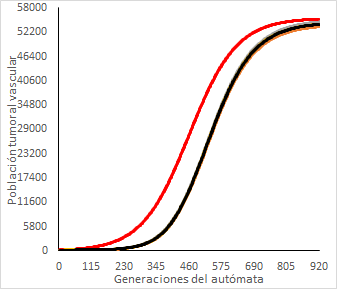
\includegraphics{img/graphs/graph-vascular-simulations-pro-1.png}}
\scalebox{0.8}{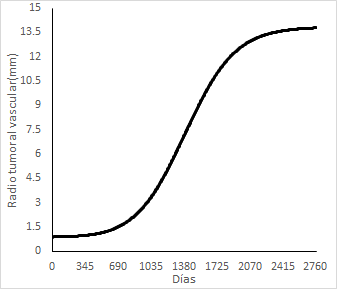
\includegraphics{img/graphs/graph-vascular-simulations-pro-r-1.png}}}\vspace*{-0.2cm}
\subfigure[Crecimiento m\'aximo $K_v=1$.$111 \times 10^5$]{\scalebox{0.8}{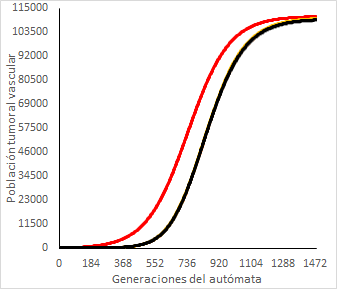
\includegraphics{img/graphs/graph-vascular-simulations-max-1.png}}
\scalebox{0.8}{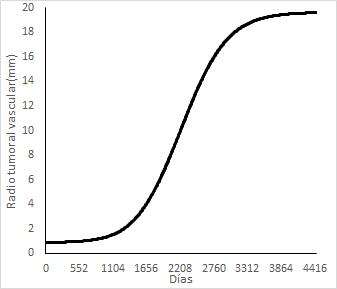
\includegraphics{img/graphs/graph-vascular-simulations-max-r-1.png}}}\vspace*{-0.2cm}
\end{center}\vspace*{-0.6cm}
\caption[Poblaci\'on y radios de un carcinoma ductal infiltrante de crecimiento lento con $\rho_{max}^v=0$.$1$ durante la etapa vascular]{Poblaci\'on y radios de un carcinoma ductal infiltrante de crecimiento lento con $\rho_{max}^v=0$.$1$ durante la etapa vascular. El resto de par\'ametros se muestran en el cuadro~\ref{table-vascular-1}. (a,b,c--izquierda) En rojo los valores obtenidos de la soluci\'on de la ley de crecimiento log\'istico, en negro los promedios de la poblaci\'on tumoral y el resto de curvas son varias simulaciones del aut\'omata. (a,b,c--derecha) En negro los promedios del radio tumoral.}
\label{graph-vascular-simulations-1}
\end{figure}

Con el objetivo de establecer comparaciones se determina un conjunto de par\'ametros del modelo de crecimiento log\'istico que describen el desarrollo de un tumor vascular de crecimiento lento. Para ello se utilizan los valores de la poblaci\'on inicial y de las capacidades de carga m\'inimas, promedio y m\'aximas correspondientes con el intervalo de radios vasculares $R_v \in [10, 15]mm$ y una probabilidad m\'axima avascular $\rho_{max}^v=0$.$1$ como se muestra en el cuadro~\ref{table-vascular-1}. El modelo puede reproducir tumores que toman mucho m\'as tiempo para su desarrollo pero se considera adecuado mostrar el crecimiento para la anterior probabilidad m\'axima $\rho_{max}^v=0$.$1$ para establecer dichas comparaciones; e.g. tumores con una probabilidad m\'axima menor como $\rho_{max}^v=0$.$01$. Los resultados provenientes de las simulaciones con los par\'ametros del cuadro~\ref{table-vascular-1} se muestran en las gr\'aficas~\ref{graph-vascular-simulations-1}. El an\'alisis de los resultados presentados se lleva a cabo en la secci\'on~\ref{sec-growth-validation}.
\begin{table}[!ht]
\begin{center}
\scalebox{0.9}{\begin{tabular}{|p{2.1cm}|p{14.5cm}|}\hline
\emph{M\'inimo} & $P_0^v=2$.$222 \times 10^2$, $K_v=2$.$778 \times 10^4$, $r_v=1$.$44 \times 10^{-5}$, $\Delta t=1$.$187 \times 10^3$, generaciones del aut\'omata: $565$~($1695$ d\'ias).\\\hline
\emph{Promedio} & $P_0^v=2$.$222 \times 10^2$, $K_v=5$.$556 \times 10^4$, $r_v=7$.$199 \times 10^{-6}$, $\Delta t=1$.$659 \times 10^3$, generaciones del aut\'omata: $925$~($2775$ d\'ias).\\\hline
\emph{M\'aximo} & $P_0^v=2$.$222 \times 10^2$, $K_v=1$.$111 \times 10^5$, $r_v=8$.$097 \times 10^{-3}$, $\Delta t=4$.$558 \times 10^1$, generaciones del aut\'omata: $1481$~($4443$ d\'ias).\\\hline
\end{tabular}}\vspace*{-0.6cm}
\end{center}
\caption[Par\'ametros del desarrollo de un carcinoma ductal infiltrante de crecimiento lento durante la etapa vascular]{Par\'ametros del desarrollo de un carcinoma ductal infiltrante de crecimiento lento durante la etapa vascular.}
\label{table-vascular-1}
\end{table}

En la figura~\ref{fig-vascular-automata} se muestran las visualizaciones de una de las simulaciones del aut\'omata de un tumor vascular de crecimiento r\'apido. En estas visualizaciones no se muestran poblaciones de c\'elulas migratorias ni de micromet\'astasis porque estas reglas no fueron evaluadas durante estas simulaciones con el objetivo de mostrar solamente el crecimiento vascular del tumor. Se puede apreciar un aumento considerable de la poblaci\'on tumoral, as\'i como la invasi\'on del estroma que avanza progresivamente a medida que avanza su desarrollo. En las gr\'aficas para el crecimiento vascular no es posible apreciar correctamente las curvas correspondientes con varias simulaciones del aut\'omata pues son en extremo cercanas a la curva que representa el promedio.
\begin{figure}[!ht]
\begin{center}
\subfigure[Generaci\'on 0]{\scalebox{0.29}{
\includegraphics{img/automata/201951822631-22.png}}}
\subfigure[Generaci\'on 40]{\scalebox{0.29}{
\includegraphics{img/automata/201951822631-62.png}}}
\subfigure[Generaci\'on 80]{\scalebox{0.29}{
\includegraphics{img/automata/201951822631-102.png}}}\vspace*{-0.25cm}
\subfigure[Generaci\'on 120]{\scalebox{0.29}{
\includegraphics{img/automata/201951822631-142.png}}}
\subfigure[Generaci\'on 160]{\scalebox{0.29}{
\includegraphics{img/automata/201951822631-182.png}}}
\subfigure[Generaci\'on 200]{\scalebox{0.29}{
\includegraphics{img/automata/201951822631-221.png}}}\vspace*{-0.25cm}
\end{center}\vspace*{-0.6cm}
\caption[Visualizaciones de una simulaci\'on del aut\'omata celular de un carcinoma ductal infiltrante de crecimiento r\'apido durante la etapa vascular]{Visualizaciones de una simulaci\'on del aut\'omata celular de un carcinoma ductal infiltrante de crecimiento r\'apido durante la etapa vascular. Las generaciones del aut\'omata mostradas se obtienen mediante los par\'ametros correspondientes con la capacidad de carga promedio~(cuadro~\ref{table-vascular}) y se toman relativas al inicio de dicha etapa. El \'area mostrada posee dimensiones $[0,52$.$5]mm \times [0,52$.$5]mm$.}
\label{fig-vascular-automata}
\end{figure}

\section{Validaci\'on del crecimiento tumoral}
\label{sec-growth-validation}
Como se pudo apreciar en los datos obtenidos de la simulaci\'on del crecimiento tumoral durante las etapas avascular y vascular la curva descrita por la utilizaci\'on de la ecuaci\'on de crecimiento log\'istica posee la forma caracter\'istica de \emph{S}~\cite{book} presente en otros modelos de la literatura que utilizan otras ecuaciones de crecimiento como Gompertz~\cite{kansal,dormann,kansal2,kansal3}, en las que el crecimiento se divide en tres etapas representativas: una fase inicial pasiva, una fase intermedia de crecimiento exponencial y una fase final de ralentizaci\'on. Estas tres etapas se evidencian claramente en las gr\'aficas~\ref{graph-avascular-simulations}, \ref{graph-avascular-simulations-1}, \ref{graph-vascular-simulations} y \ref{graph-vascular-simulations-1} provenientes de las simulaciones computacionales del modelo. Las ejecuciones del aut\'omata celular reproducen el crecimiento log\'istico con diferencias causadas principalmente por la naturaleza desigual de ambos modelos. Las causas que se listan a continuaci\'on se aplican a las diferencias entre la ley de crecimiento log\'istico y el modelo de aut\'omatas celulares concebido tanto durante la etapa avascular como durante la vascular: la influencia de los vectores de concentraci\'on~($\beta_{tum}(v,l)$), la influencia de la velocidad de expansi\'on~($\gamma_{tum}(v,N(v,l))$) y el error de aproximaci\'on proveniente del uso de la escala $1:3$.

Durante la realizaci\'on de las simulaciones computacionales se comprob\'o que el modelo devuelve valores biol\'ogicamente realistas, tanto en el tiempo como en las cantidades de c\'elulas cancer\'igenas presentes en ambas etapas del crecimiento. En cuanto al tiempo el $50\%$ de los casos de carcinomas se consideran tumores de crecimiento r\'apido y se desarrollan en un lapso de $1$--$2$ a\~nos, el $33\%$ de los casos se consideran tumores de crecimiento intermedio y se desarrollan en un lapso de $2$--$5$ a\~nos, y cerca del $17\%$ de los casos se consideran tumores de crecimiento lento desarroll\'andose todo el ciclo tumoral en un lapso mayor de $5$ a\~nos pr\'acticamente sin l\'imite de tiempo~\cite{nakashima,leekim,sopik}. Los casos extremos mostrados anteriormente para ambas etapas demuestran que el modelo es capaz de reconstruir el desarrollo tumoral para un per\'iodo de tiempo arbitrario; e.g. si se desea reproducir el desarrollo de un tumor de crecimiento r\'apido se pueden combinar los par\'ametros de ambas etapas para este tipo de tumores obteni\'endose todo el ciclo vital tumoral en un lapso de $27$ d\'ias para la etapa avascular y $423$ d\'ias para la etapa vascular. Este lapso de tiempo coincide con un per\'iodo de un a\~no entrando en la categor\'ia de carcinoma de crecimiento r\'apido como se expuso al comienzo de este p\'arrafo.

En cuanto a los radios y las poblaciones se puede apreciar que se obtienen los valores establecidos con anterioridad en la secci\'on~\ref{subsec-network-param}, con un crecimiento avascular variable entre $0$.$5mm$ y $1mm$, y un crecimiento vascular variable entre $10mm$ y $15mm$ como se aprecia en las gr\'aficas. Las diferencias entre los valores del radio encontrados durante la etapa avascular se deben a las causas listadas al comienzo de la presente secci\'on, principalmente el uso de la escala que provoca una sobreestimaci\'on del valor del radio. Como se expuso en la secci\'on~\ref{subsec-scale-param} cuando se utiliza la escala de la simulaci\'on se asume que una celda del aut\'omata que posee los estados correspondientes con una c\'elula tumoral o de una micromet\'astasis se encuentra totalmente ocupada por c\'elulas de esos tipos. Esto no siempre se cumple para las celdas m\'as externas pertenecientes a una neoplasia. Por tanto existe una cantidad de c\'elulas de la neoplasia para las que se est\'an contabilizando una mayor cantidad de c\'elulas cancer\'igenas de las que existen en una simulaci\'on a escala $1:1$, lo que constituye el origen de la sobreestimaci\'on. En la etapa vascular esta sobreestimaci\'on es mucho menor ya que al aumentar los valores de la poblaci\'on el error de aproximaci\'on se vuelve inferior. Esta deficiencia debe ser corregida en trabajos futuros. Siguiendo el ejemplo anterior de la reconstrucci\'on del desarrollo tumoral combinando par\'ametros de ambas etapas es posible obtener valores del radio de $0$.$5mm$ para la etapa avascular y partiendo de este valor obtener un radio de $10mm$ para la etapa vascular.

\begin{figure}[p]
\begin{center}
\subfigure[Etapa avascular $r_a \approx 0$.$5mm$]{\scalebox{0.8}{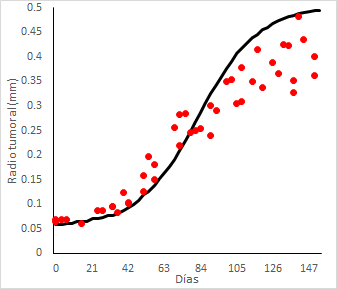
\includegraphics{img/graphs/graph-validation-1.png}}}
\subfigure[Etapa avascular $r_a \approx 0$.$75mm$]{\scalebox{0.8}{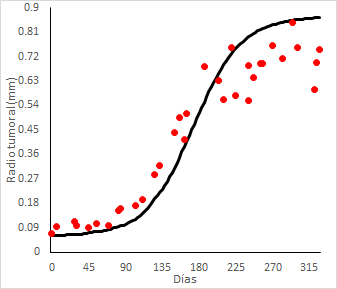
\includegraphics{img/graphs/graph-validation-2.png}}}\vspace*{-0.2cm}
\subfigure[Etapa avascular $r_a \approx 1$.$0mm$]{\scalebox{0.8}{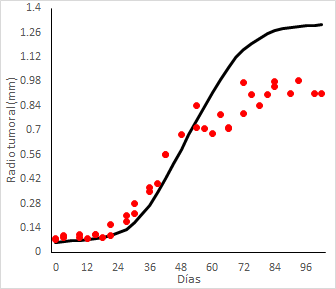
\includegraphics{img/graphs/graph-validation-3.png}}}
\subfigure[Etapa vascular $r_v \approx 10mm$]{\scalebox{0.8}{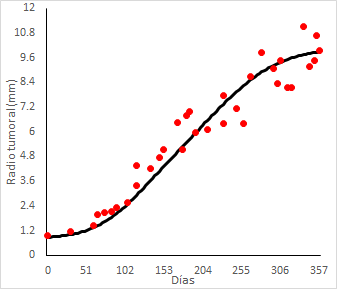
\includegraphics{img/graphs/graph-validation-4.png}}}\vspace*{-0.2cm}
\subfigure[Etapa vascular $r_v \approx 15mm$]{\scalebox{0.8}{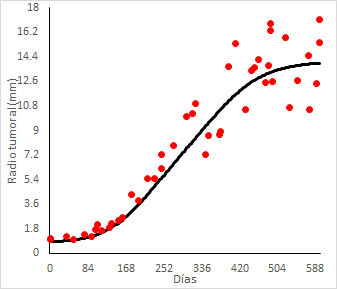
\includegraphics{img/graphs/graph-validation-5.png}}}
\subfigure[Etapa vascular $r_v \approx 20mm$]{\scalebox{0.8}{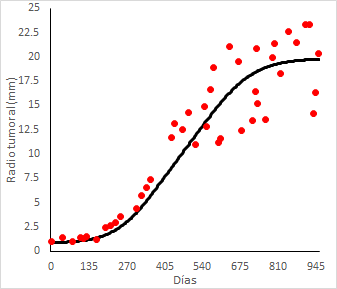
\includegraphics{img/graphs/graph-validation-6.png}}}\vspace*{-0.2cm}
\end{center}\vspace*{-0.6cm}
\caption[Comparaci\'on entre los radios de carcinomas ductales infiltrantes obtenidos de observaciones cl\'inicas y del modelo]{Comparaci\'on entre los radios de carcinomas ductales infiltrantes obtenidos de observaciones cl\'inicas~\cite{wisconsin,wisconsindata,kuhn,helmlinger} y del modelo. En negro se muestra el radio tumoral obtenido del modelo mientras que los puntos se corresponden con observaciones en las que el tumor analizado alcanza valores pr\'oximos a los mostrados en los casos extremos en tiempos similares.}
\label{graph-growth-validation}
\end{figure}

Utilizando la informaci\'on de diversos sitios y trabajos disponibles~\cite{wisconsin,wisconsindata,kuhn,helmlinger} se extrajeron varios datos de observaciones del desarrollo tumoral en el tiempo utilizando el radio como medio de comparaci\'on. Las observaciones que fueron seleccionadas se corresponden con tumores que alcanzaron radios m\'aximos pr\'oximos a los mostrados en los casos extremos en tiempos similares. La realizaci\'on de estas comparaciones es una tarea que no se encuentra libre de errores de aproximaci\'on causados principalmente por la suposici\'on de la esfericidad como justificaci\'on para el uso del radio como medida de la dimensi\'on del tumor. Si se presenta un caso correspondiente con un tumor vascular se toma como radio inicial $1mm$ y el tiempo se toma relativo al tiempo de las mediciones. Las comparaciones se muestran en las gr\'aficas~\ref{graph-growth-validation}. 

Las diferencias entre las observaciones y los radios mostrados se debe a la variaci\'on del tiempo que le toma a un tumor duplicar su volumen. Este valor no es constante y var\'ia en dependencia de numerosos factores como las cantidades de nutrientes, la compresi\'on mec\'anica del entorno, la presencia de factores de crecimiento entre otras muchas que no pueden representarse en un modelo de crecimiento tan simple como el utilizado en este trabajo~\cite{robins,nakashima}. Tambi\'en es posible que entre observaciones el radio tumoral disminuya producto de la acci\'on del sistema inmunitario, comportamiento que nuestro modelo no puede representar por tratarse de un proceso de crecimiento simple. Destaquemos que otros modelos presentes en la literatura presentan los mismos problemas mencionados~\cite{kansal,dormann}. Esta conclusi\'on es la esperada, pues constituye un objetivo a conseguir en trabajos futuros. A pesar de los aspectos negativos citados el modelo reproduce con suficiente precisi\'on el crecimiento tumoral. Se aprecia en las gr\'aficas~\ref{graph-growth-validation}a, \ref{graph-growth-validation}b y \ref{graph-growth-validation}c el desajuste causado por la sobreestimaci\'on del radio durante la etapa avascular.

\section{Aparici\'on de c\'elulas migratorias}
\label{sec-migra-app-results}
En las secciones anteriores se presentaron diversos grupos de par\'ametros de la ley de crecimiento log\'istico para ambas etapas del desarrollo tumoral. Siguiendo la idea de mostrar dos casos extremos reproducidos por el modelo partimos de un tumor primario que presenta una aparici\'on temprana con una tasa de producci\'on de c\'elulas migratorias alta, me refiero a los par\'ametros $\eta_{mig}$ y $K_{mig}$. Para mostrar estos comportamientos establecemos par\'ametros base para la propia migraci\'on: $\mu_{mig}=1$, $\mu_{max}=55$ y $\eta_{mig}'=0$.$1$, que ser\'an analizados m\'as adelante, y se utilizan los par\'ametros de la ley de crecimiento log\'istico de un tumor de r\'apido crecimiento para ambas etapas con capacidades de carga promedio. El primer grupo de par\'ametros se muestran en el cuadro~\ref{table-migra} con una probabilidad m\'axima de aparici\'on de $0$.$1$. En cuanto a la cantidad de generaciones del aut\'omata se toman: $20$ generaciones de la etapa avascular, $200$ generaciones de la etapa vascular y $100$ generaciones adicionales para recolectar los datos de la aparici\'on de c\'elulas migratorias, para un total de $320$ generaciones correspondientes con $960$ d\'ias o $2$ a\~nos y medio aproximadamente. En la figura~\ref{graph-migra-app} se aprecian las gr\'aficas correspondientes con la producci\'on de c\'elulas migratorias y la cantidad de estas c\'elulas activas por generaci\'on. En la figura~\ref{fig-migra-automata} se muestran las visualizaciones del aut\'omata, en las que se han ampliado las c\'elulas migratorias para una mejor apreciaci\'on. Como se puede apreciar en las gr\'aficas se detectaron surgimientos de estas c\'elulas en la generaci\'on $23$ del aut\'omata aproximadamente, apenas $9$ d\'ias despu\'es de abandonar la etapa avascular. 
\begin{table}[!ht]
\begin{center}
\scalebox{0.9}{\begin{tabular}{|p{2.1cm}|p{14.5cm}|}\hline
\emph{Migraci\'on} & Aparici\'on de c\'elulas migratorias -- $\eta_{mig}=1$, $K_{mig}=5$.$0 \times 10^5$, probabilidad de aparici\'on $0$.$1$.\\\hline
\end{tabular}}\vspace*{-0.6cm}
\end{center}
\caption[Par\'ametros de la regla de la aparici\'on de c\'elulas migratorias de un carcinoma ductal infiltrante con alta tasa de producci\'on y aparici\'on temprana]{Par\'ametros de la regla de la aparici\'on de c\'elulas migratorias de un carcinoma ductal infiltrante con alta tasa de producci\'on y aparici\'on temprana.}
\label{table-migra}
\end{table}

\begin{figure}[p]
\begin{center}
\subfigure[Producci\'on de c\'elulas migratorias]{\scalebox{0.8}{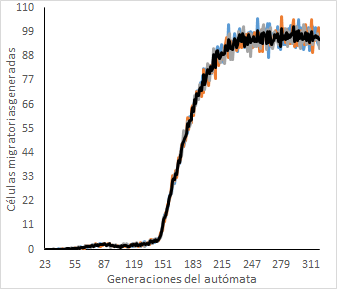
\includegraphics{img/graphs/graph-migra-app.png}}}
\subfigure[Cantidad de c\'elulas migratorias activas]{\scalebox{0.8}{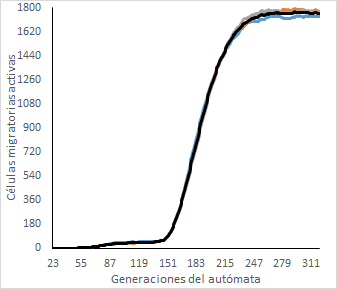
\includegraphics{img/graphs/graph-migra-act.png}}}\vspace*{-0.25cm}
\end{center}\vspace*{-0.6cm}
\caption[Gr\'aficas de la producci\'on y cantidades activas de c\'elulas migratorias de un carcinoma ductal infiltrante con una alta tasa de producci\'on y aparici\'on temprana]{Gr\'aficas de la producci\'on y cantidades activas de c\'elulas migratorias de un carcinoma ductal infiltrante con una alta tasa de producci\'on y aparici\'on temprana. Estos datos se obtienen utilizando los par\'ametros mostrados en el cuadro~\ref{table-migra}. (a) Curvas de la cantidad de c\'elulas migratorias producidas por generaci\'on en varias simulaciones del aut\'omata y su promedio~(en negro). (b) Curvas de la cantidad de c\'elulas migratorias activas por generaci\'on en varias simulaciones del aut\'omata y su promedio~(en negro).}
\label{graph-migra-app}
\end{figure}

\begin{figure}[p]
\begin{center}
\subfigure[Generaci\'on 23]{\scalebox{0.29}{
\includegraphics{img/automata/2019519174453-23.png}}}
\subfigure[Generaci\'on 82]{\scalebox{0.29}{
\includegraphics{img/automata/2019519174453-82.png}}}
\subfigure[Generaci\'on 141]{\scalebox{0.29}{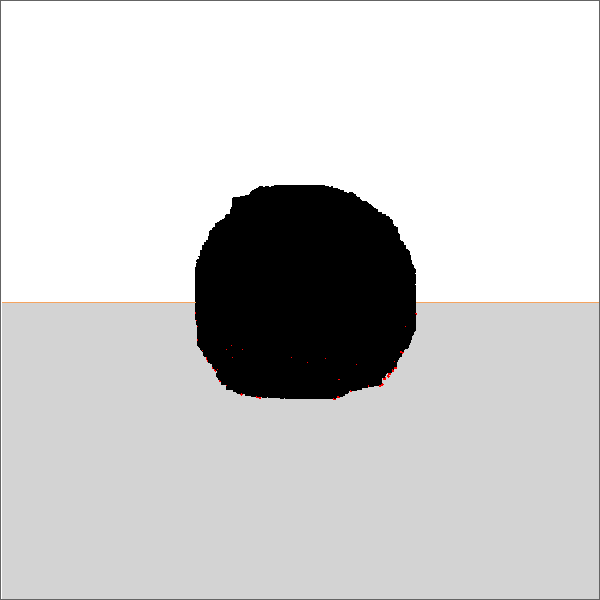
\includegraphics{img/automata/2019519174453-141.png}}}\vspace*{-0.25cm}
\subfigure[Generaci\'on 200]{\scalebox{0.29}{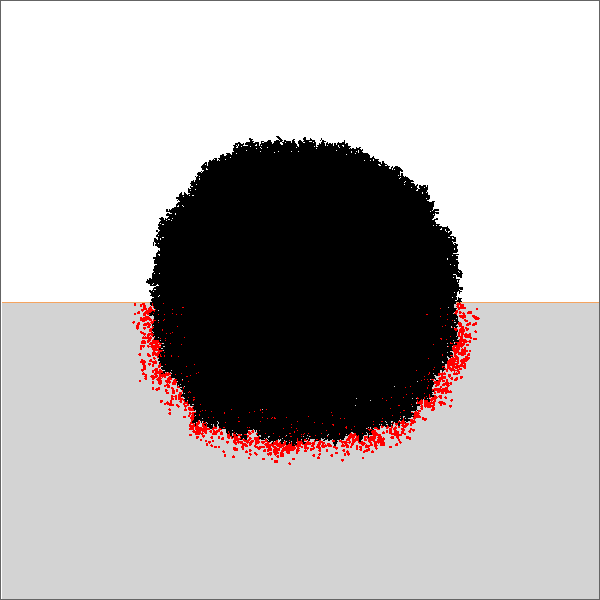
\includegraphics{img/automata/2019519174453-200.png}}}
\subfigure[Generaci\'on 259]{\scalebox{0.29}{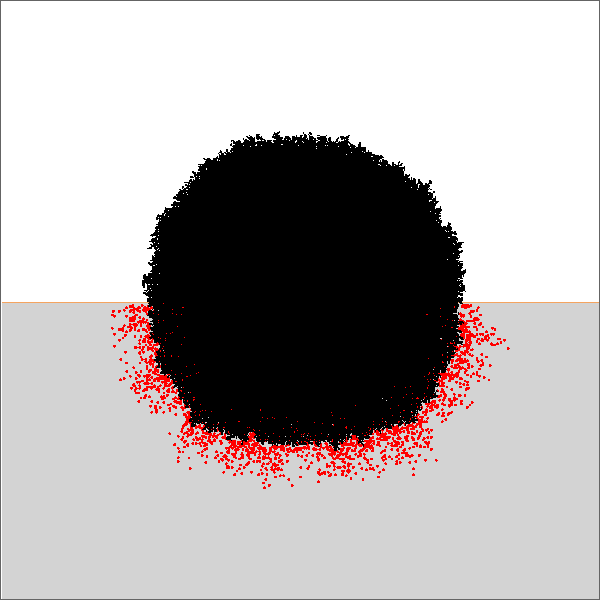
\includegraphics{img/automata/2019519174453-259.png}}}
\subfigure[Generaci\'on 318]{\scalebox{0.29}{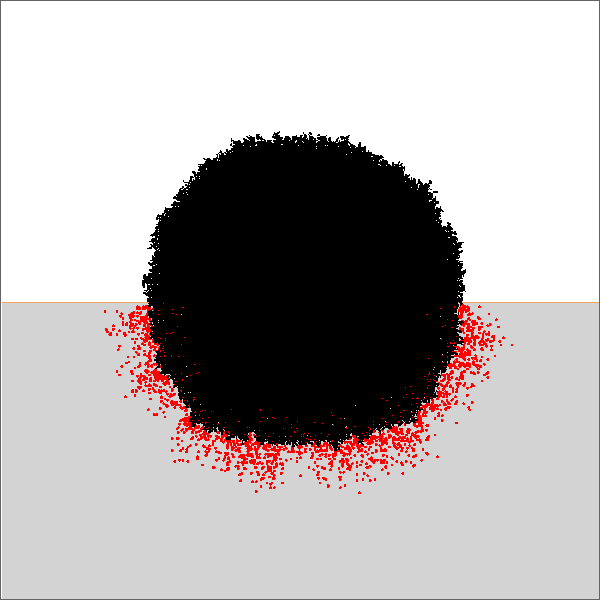
\includegraphics{img/automata/2019519174453-318.png}}}\vspace*{-0.25cm}
\end{center}\vspace*{-0.6cm}
\caption[Visualizaciones de una simulaci\'on del aut\'omata celular donde se aprecia la aparici\'on de c\'elulas migratorias de un carcinoma ductal infiltrante con alta tasa de producci\'on y aparici\'on temprana]{Visualizaciones de una simulaci\'on del aut\'omata celular donde se aprecia la aparici\'on de c\'elulas migratorias de un carcinoma ductal infiltrante con alta tasa de producci\'on y aparici\'on temprana. Las generaciones del aut\'omata fueron obtenidas mediante el uso de los par\'ametros mostrados en el cuadro~\ref{table-migra}. El \'area mostrada posee dimensiones $[0,52$.$5]mm \times [0,52$.$5]mm$.}
\label{fig-migra-automata}
\end{figure}

El segundo grupo de par\'ametros de la aparici\'on de c\'elulas migratorias se corresponden con un tumor que presenta una baja tasa de producci\'on y aparici\'on tard\'ia de dichas c\'elulas. En este caso se mantienen las mismas cantidades de generaciones para el aut\'omata al igual que los par\'ametros para el crecimiento tumoral en ambas etapas: $20$ generaciones de la etapa avascular, $200$ generaciones de la etapa vascular y $100$ generaciones adicionales para recolectar los datos de la aparici\'on de c\'elulas migratorias. Los par\'ametros se muestran en el cuadro~\ref{table-migra-1} con una probabilidad m\'axima de aparici\'on de $0$.$01$. En la figura~\ref{graph-migra-app-1} se aprecian las gr\'aficas correspondientes con la producci\'on de c\'elulas migratorias y la cantidad de estas c\'elulas activas por generaci\'on. En la figura~\ref{fig-migra-automata-1} se muestran las visualizaciones del aut\'omata, en las que se han ampliado las c\'elulas migratorias~(en rojo) para una mejor apreciaci\'on. Como se puede apreciar en las gr\'aficas estas c\'elulas comienzan su aparici\'on aproximadamente en la generaci\'on $99$ del aut\'omata, $237$ d\'ias despu\'es de abandonar la etapa avascular. 
\begin{table}[!ht]
\begin{center}
\scalebox{0.9}{\begin{tabular}{|p{2.1cm}|p{14.5cm}|}\hline
\emph{Migraci\'on} & Aparici\'on de c\'elulas migratorias -- $\eta_{mig}=0$.$1$, $K_{mig}=3$.$249 \times 10^4$, probabilidad de aparici\'on $0$.$01$.\\\hline
\end{tabular}}\vspace*{-0.6cm}
\end{center}
\caption[Par\'ametros de la regla de la aparici\'on de c\'elulas migratorias de un carcinoma ductal infiltrante con una baja tasa de producci\'on y aparici\'on tard\'ia]{Par\'ametros de la regla de la aparici\'on de c\'elulas migratorias de un carcinoma ductal infiltrante con una baja tasa de producci\'on y aparici\'on tard\'ia.}
\label{table-migra-1}
\end{table}

\begin{figure}[p]
\begin{center}
\subfigure[Producci\'on de c\'elulas migratorias]{\scalebox{0.8}{\includegraphics{img/graphs/graph-migra-app-1.png}}}
\subfigure[Cantidad de c\'elulas migratorias activas]{\scalebox{0.8}{\includegraphics{img/graphs/graph-migra-act-1.png}}}\vspace*{-0.25cm}
\end{center}\vspace*{-0.6cm}
\caption[Gr\'aficas de la aparici\'on y cantidades activas de c\'elulas migratorias de un carcinoma ductal infiltrante con una baja tasa de producci\'on y aparici\'on tard\'ia]{Gr\'aficas de la aparici\'on y cantidades activas de c\'elulas migratorias de un carcinoma ductal infiltrante con una baja tasa de producci\'on y aparici\'on tard\'ia. Estos datos se obtienen utilizando los par\'ametros mostrados en el cuadro~\ref{table-migra-1}. (a) Curvas de la cantidad de c\'elulas migratorias producidas por generaci\'on en varias simulaciones del aut\'omata y su promedio~(en negro). (b) Curvas de la cantidad de c\'elulas migratorias activas por generaci\'on en varias simulaciones del aut\'omata y su promedio~(en negro).}
\label{graph-migra-app-1}
\end{figure}

\begin{figure}[p]
\begin{center}
\subfigure[Generaci\'on 99]{\scalebox{0.29}{\includegraphics{img/automata/201951919754-99.png}}}
\subfigure[Generaci\'on 143]{\scalebox{0.29}{\includegraphics{img/automata/201951919754-143.png}}}
\subfigure[Generaci\'on 187]{\scalebox{0.29}{\includegraphics{img/automata/201951919754-187.png}}}\vspace*{-0.25cm}
\subfigure[Generaci\'on 231]{\scalebox{0.29}{\includegraphics{img/automata/201951919754-231.png}}}
\subfigure[Generaci\'on 275]{\scalebox{0.29}{\includegraphics{img/automata/201951919754-275.png}}}
\subfigure[Generaci\'on 319]{\scalebox{0.29}{\includegraphics{img/automata/201951919754-319.png}}}\vspace*{-0.25cm}
\end{center}\vspace*{-0.6cm}
\caption[Visualizaciones de una simulaci\'on del aut\'omata celular donde se aprecia la aparici\'on de c\'elulas migratorias de un carcinoma ductal infiltrante con una baja tasa de producci\'on y aparici\'on tard\'ia]{Visualizaciones de una simulaci\'on del aut\'omata celular donde se aprecia la aparici\'on de c\'elulas migratorias de un carcinoma ductal infiltrante con una baja tasa de producci\'on y aparici\'on tard\'ia. Las generaciones del aut\'omata fueron obtenidas mediante el uso de los par\'ametros mostrados en el cuadro~\ref{table-migra-1}. El \'area mostrada posee dimensiones $[0,52$.$5]mm \times [0,52$.$5]mm$.}
\label{fig-migra-automata-1}
\end{figure}

\section{Migraci\'on}
\label{sec-migra-mov-results}
En esta secci\'on se presentan los casos extremos correspondientes con la extensi\'on de la migraci\'on, es decir, la distancia que pueden recorrer las c\'elulas migratorias desde la frontera tumoral hasta un posible punto de intravasaci\'on o su muerte celular. Siguiendo la idea de la secci\'on anterior estableceremos valores base para el grupo de par\'ametros que controla la aparici\'on de c\'elulas migratorias $\eta_{mig}=0$.$5$ y $K_{mig}=1$.$929 \times 10^5$ con una probabilidad m\'axima de aparici\'on de $0$.$05$. En cuanto al crecimiento se utilizan los par\'ametros correspondientes con un tumor de r\'apido crecimiento en ambas etapas con capacidades de carga promedio. En la secci\'on~\ref{subsec-model-param} se expuso que la distancia que puede migrar una c\'elula cancer\'igena oscila entre $1mm$ y $10mm$, lo que se traduce en un rango de desplazamientos tentativos de $[10,100]$ ajustado a la escala $1:3$. Los par\'ametros $\eta_{mig}'$ y $\mu_{mig}$ se utilizan con sus valores por defecto $0$.$1$ y $1$ respectivamente. Se muestran tres casos a diferencia de las secciones anteriores porque el caso promedio es necesario para mostrar la transici\'on de los datos extra\'idos de este comportamiento. Los par\'ametros se muestran en el cuadro~\ref{table-migra-mov}. Las gr\'aficas~\ref{graph-migra-mov} muestran los promedios de las cantidades de c\'elulas contra la cantidad de desplazamientos realizados que culminan en muerte celular o en intravasaci\'on. En la figura~\ref{fig-migra-mov} se muestran visualizaciones de la generaci\'on $320$ para cada caso extremo.
\begin{table}[!ht]
\begin{center}
\scalebox{0.9}{\begin{tabular}{|p{2.1cm}|p{14.5cm}|}\hline
\emph{Migraci\'on} & $\mu_{mig}=1$, $\eta_{mig}'=0$.$1$, desplazamiento m\'aximo -- $\mu_{max}=100$, desplazamiento promedio -- $\mu_{max}=55$, desplazamiento m\'inimo -- $\mu_{max}=10$.\\\hline
\end{tabular}}\vspace*{-0.6cm}
\end{center}
\caption[Par\'ametros de la regla de la migraci\'on de c\'elulas cancer\'igenas de un carcinoma ductal infiltrante]{Par\'ametros de la regla de la migraci\'on de c\'elulas cancer\'igenas de un carcinoma ductal infiltrante.}
\label{table-migra-mov}
\end{table}

\begin{figure}[p]
\begin{center}
\subfigure[$\mu_{max}=100$]{\scalebox{0.8}{\includegraphics{img/graphs/graph-migra-desp-death.png}}
\scalebox{0.8}{\includegraphics{img/graphs/graph-migra-desp-metas.png}}}\vspace*{-0.25cm}
\subfigure[$\mu_{max}=55$]{\scalebox{0.8}{\includegraphics{img/graphs/graph-migra-desp-death-1.png}}
\scalebox{0.8}{\includegraphics{img/graphs/graph-migra-desp-metas-1.png}}}\vspace*{-0.25cm}
\subfigure[$\mu_{max}=10$]{\scalebox{0.8}{\includegraphics{img/graphs/graph-migra-desp-death-2.png}}
\scalebox{0.8}{\includegraphics{img/graphs/graph-migra-desp-metas-2.png}}}\vspace*{-0.25cm}
\end{center}\vspace*{-0.6cm}
\caption[Gr\'aficas de la cantidad de desplazamientos llevados a cabo por c\'elulas migratorias]{Gr\'aficas de la cantidad de desplazamientos llevados a cabo por c\'elulas migratorias para los valores de $\mu_{max}$ indicados. Estos datos se obtienen utilizando los par\'ametros mostrados en el cuadro~\ref{table-migra-mov}. (a,b,c-izquierda) Promedios de la cantidad de c\'elulas que terminan su existencia durante la migraci\'on. (a,b,c-derecha) Promedios de la cantidad de c\'elulas que culminan su migraci\'on penetrando el sistema circulatorio.}
\label{graph-migra-mov}
\end{figure}

\begin{figure}[!ht]
\begin{center}
\scalebox{0.29}{\includegraphics{img/automata/201952101815-320.png}}
\scalebox{0.29}{\includegraphics{img/automata/20195212856-320.png}}
\scalebox{0.29}{\includegraphics{img/automata/201952111416-320.png}}
\end{center}\vspace*{-0.6cm}
\caption[Visualizaciones de simulaciones del aut\'omata celular de un carcinoma ductal infiltrante donde se aprecian distintas distancias m\'aximas de la migraci\'on]{Visualizaciones de simulaciones del aut\'omata celular de un carcinoma ductal infiltrante donde se aprecian distintas distancias m\'aximas de la migraci\'on. Se obtuvieron mediante el uso de los par\'ametros mostrados en el cuadro~\ref{table-migra-mov}. El \'area mostrada posee dimensiones $[0,52$.$5]mm \times [0,52$.$5]mm$.}
\label{fig-migra-mov}
\end{figure}

\section{Discusi\'on de la migraci\'on}
\label{sec-migra-validation}
Como verificaci\'on de la reproducci\'on satisfactoria del proceso migratorio en el presente modelo se muestran en la figura~\ref{fig-migra-kansal3} una visualizaci\'on de nuestro modelo y de una imagen tomada del trabajo~\cite{kansal3} donde se evidencia la aparici\'on de estas ramas formadas por c\'elulas migratorias que ocurren en todas las formas de c\'ancer invasivo. Las distancias recorridas en estas im\'agenes no pueden utilizarse como validaci\'on pues se trata de tipos de c\'ancer distintos y de condiciones distintas, en nuestro caso el modelo est\'a pensado para reproducir el crecimiento natural del c\'ancer mientras que la imagen tomada de~\cite{kansal3} se corresponden con un MTS cultivado \emph{in vitro}. Estos cultivos se realizan en el interior de un gel de agarosa~\cite{helmlinger} por lo que la formaci\'on de ramas invasivas ocurre en todas las direcciones, a diferencia de lo que ocurre en un tumor que surge en el epitelio donde estas ramas invasivas solo pueden crecer en direcci\'on al estroma.
\begin{figure}[!ht]
\begin{center}
\scalebox{0.29}{\includegraphics{img/automata/2019519174453-318.png}}\hspace*{0.5cm}
\scalebox{0.47}{\includegraphics{img/fig-kansal3-mets.png}}
\end{center}\vspace*{-0.5cm}
\caption[Comparaci\'on entre las visualizaciones del modelo del presente manuscrito y de una imagen microsc\'opica de un glioblastoma multiforme]{Comparaci\'on entre las visualizaciones del modelo del presente manuscrito y de una imagen microsc\'opica de un glioblastoma multiforme~(Figura tomada de~\cite{kansal3}).}
\label{fig-migra-kansal3}
\end{figure}

Como se pudo apreciar en las gr\'aficas~\ref{graph-migra-app} y~\ref{graph-migra-app-1} a partir de una generaci\'on espec\'ifica, en ambos casos ocurre aproximadamente en la generaci\'on $225$, se alcanza un equilibrio en la producci\'on y en la cantidad de c\'elulas migratorias activas. Este equilibro se logra mediante tres factores fundamentales. El ritmo de producci\'on depende de la funci\'on de probabilidad de aparici\'on de c\'elulas migratorias $\rho_2(n_i \rightarrow 4)$ que alcanza su m\'aximo cuando la poblaci\'on estimada del tumor se acerca a su m\'aximo. Como la poblaci\'on tumoral se mantiene casi constante en su valor m\'aximo, aproximadamente $K_v$, la probabilidad de aparici\'on de c\'elulas migratorias se vuelve una constante, aproximadamente el valor establecido previamente. La migraci\'on de las c\'elulas cercanas a la frontera es crucial para que se alcance este equilibrio ya que libera celdas del aut\'omata que pueden ser ocupadas por nuevas c\'elulas migratorias en generaciones posteriores. El ritmo de muerte de las c\'elulas migratorias cuando se aproximan a la distancia m\'axima recorrida influye en la cantidad de c\'elulas migratorias activas. Si dicha distancia m\'axima se hace mayor se espera que la cantidad de c\'elulas migratorias activas aumente.

En estas gr\'aficas~\ref{graph-migra-app} y~\ref{graph-migra-app-1} tambi\'en se puede apreciar el hecho de que la producci\'on de c\'elulas migratorias aumenta considerablemente pasado un punto espec\'ifico, en ambos casos ocurre aproximadamente en la generaci\'on $151$, que coincide con el momento en que la velocidad de expansi\'on del tumor comienza a disminuir. Esta velocidad depende de la probabilidad del crecimiento tumoral, que como se expuso en la secci\'on~\ref{subsec-migrant} posee prioridad sobre la aparici\'on de c\'elulas migratorias. A medida que el ritmo del crecimiento tumoral disminuye se vuelve m\'as probable la aparici\'on de una c\'elula migratoria. El segundo motivo para este comportamiento tiene que ver con la velocidad de las c\'elulas migratorias. Hasta ese momento la velocidad de una c\'elula migratoria y la velocidad expansiva tumoral ten\'ian valores similares por los par\'ametros utilizados, alrededor de una celda del aut\'omata cada $72$ horas para ambos haciendo que las c\'elulas migratorias no logren aumentar la distancia entre ellas y la frontera tumoral. A medida que la velocidad de expansi\'on tumoral disminuye las c\'elulas migratorias pueden dejar atr\'as la frontera tumoral satisfactoriamente. Como es de esperarse en un tumor de crecimiento lento esto no sucede ya que la velocidad de expansi\'on ser\'a menor en todo momento que la velocidad de las c\'elulas migratorias apreci\'andose una marcada migraci\'on en todo momento. Para ilustrar esta \'ultima conclusi\'on se muestran las visualizaciones en la figura~\ref{fig-automata-superior-migra} de una simulaci\'on de un tumor de crecimiento lento durante la etapa vascular con capacidades de carga promedio, mientras que en la figura~\ref{graph-superior-migra} se muestran las gr\'aficas correspondientes con la producci\'on de c\'elulas migratorias y la cantidad de estas c\'elulas activas por generaci\'on. Si comparamos las gr\'aficas~\ref{graph-superior-migra} con las gr\'aficas~\ref{graph-migra-app} correspondientes con tumores que presentan una alta tasa de producci\'on y aparici\'on temprana de c\'elulas migratorias pero que poseen diferentes velocidades de expansi\'on durante la etapa vascular, se puede apreciar que en las primeras no existe el cambio repentino en la pendiente de las curvas mostradas en las segundas aproximadamente en la generaci\'on $151$. Este hecho se confirma con las observaciones de las visualizaciones mostradas en la figura~\ref{fig-automata-superior-migra} donde en los instantes de tiempo en que el tumor no ha alcanzado su tama\~no total se puede apreciar que la migraci\'on ocurre de forma muy marcada, en contraste con las visualizaciones mostradas en la figura~\ref{fig-migra-automata}.

\begin{figure}[p]
\begin{center}
\subfigure[Producci\'on de c\'elulas migratorias]{\scalebox{0.8}{\includegraphics{img/graphs/graph-superior-app.png}}}
\subfigure[Cantidad de c\'elulas migratorias activas]{\scalebox{0.8}{\includegraphics{img/graphs/graph-superior-act.png}}}\vspace*{-0.25cm}
\end{center}\vspace*{-0.6cm}
\caption[Gr\'aficas de la aparici\'on y cantidades activas de c\'elulas migratorias de un carcinoma ductal infiltrante de crecimiento lento con una alta tasa de producci\'on y aparici\'on temprana]{Gr\'aficas de la aparici\'on y cantidades activas de c\'elulas migratorias de un carcinoma ductal infiltrante de crecimiento lento con una alta tasa de producci\'on y aparici\'on temprana. (a) Curvas de la cantidad de c\'elulas migratorias producidas por generaci\'on en varias simulaciones del aut\'omata y su promedio~(en negro). (b) Curvas de la cantidad de c\'elulas migratorias activas por generaci\'on en varias simulaciones del aut\'omata y su promedio~(en negro).}
\label{graph-superior-migra}
\end{figure}

\begin{figure}[p]
\begin{center}
\subfigure[Generaci\'on 300]{\scalebox{0.29}{\includegraphics{img/automata/300-20195291739-Primary.png}}}
\subfigure[Generaci\'on 400]{\scalebox{0.29}{\includegraphics{img/automata/400-20195291739-Primary}}}
\subfigure[Generaci\'on 500]{\scalebox{0.29}{\includegraphics{img/automata/500-20195291739-Primary.png}}}\vspace*{-0.25cm}
\subfigure[Generaci\'on 600]{\scalebox{0.29}{\includegraphics{img/automata/600-20195291739-Primary.png}}}
\subfigure[Generaci\'on 700]{\scalebox{0.29}{\includegraphics{img/automata/700-20195291739-Primary.png}}}
\subfigure[Generaci\'on 800]{\scalebox{0.29}{\includegraphics{img/automata/800-20195291739-Primary.png}}}\vspace*{-0.25cm}
\end{center}\vspace*{-0.6cm}
\caption[Visualizaciones de simulaciones del aut\'omata celular de un carcinoma ductal infiltrante de crecimiento lento con una alta tasa de producci\'on y aparici\'on temprana]{Visualizaciones de simulaciones del aut\'omata celular de un carcinoma ductal infiltrante de crecimiento lento con una alta tasa de producci\'on y aparici\'on temprana. En los instantes de tiempo en que el tumor no ha alcanzado su tama\~no total se puede apreciar que la migraci\'on ocurre de forma muy marcada. El \'area mostrada posee dimensiones $[0,52$.$5]mm \times [0,52$.$5]mm$.}
\label{fig-automata-superior-migra}
\end{figure}

Esta conclusi\'on genera una hip\'otesis que debe ser comprobada de forma cl\'inica: para dos tumores con id\'entica capacidad para generar c\'elulas migratorias en base a sus marcadores gen\'eticos y con la misma velocidad de migraci\'on, uno con un crecimiento r\'apido y el otro un crecimiento lento, se cumplir\'a que el tumor de crecimiento lento presentar\'ia una migraci\'on muy superior al de crecimiento r\'apido. De ser cierto esta hip\'otesis constituye un posible indicador del \'area de resecci\'on necesaria para extirpar totalmente un tumor y las c\'elulas migratorias existentes en el tejido adyacente. Es un aspecto importante pues en las cirug\'ias se tiende a extraer el tumor y varios cent\'imetros adicionales de tejido para evitar dejar estas c\'elulas migratorias en el paciente, pero ocasionalmente no se cuenta con la suficiente informaci\'on para determinar el balance entre la cantidad segura de tejido a extraer y la cantidad de tejido que se desea salvar. 

El comportamiento descrito por la probabilidad de aparici\'on de c\'elulas migratorias representa un progreso en la modelaci\'on de la migraci\'on cancer\'igena, de la utilizaci\'on de una probabilidad constante~\cite{kansal3} a una probabilidad que est\'a en funci\'on del desarrollo tumoral. En los casos mostrados de la aparici\'on de c\'elulas migratorias se puede observar que dicha probabilidad aumenta conforme avanza la etapa vascular del tumor hasta alcanzar su m\'aximo valor, en estos casos $0$.$1$ y $0$.$01$. La elecci\'on de estos valores se realiz\'o en base a pruebas sucesivas y al valor utilizado en el trabajo~\cite{kansal3} donde esta probabilidad de aparici\'on de c\'elulas migratorias se conoce como \'indice mutacional y es igual a $0$.$05$, que a pesar de tratarse de un modelo de aut\'omatas para un tipo distinto de c\'ancer nos brinda una idea del rango de valores de esta probabilidad. Se observ\'o en las visualizaciones~\ref{fig-migra-automata} y~\ref{fig-migra-automata-1} que la variaci\'on de esta probabilidad altera la concentraci\'on de c\'elulas migratorias en el tejido como se puede apreciar en la figura~\ref{fig-comparisson}. Los valores de poblaciones de c\'elulas migratorias no pueden ser validados ya que no se han encontrado estudios cl\'inicos cuyo objetivo haya sido obtener estos valores. Por tanto, nuestro modelo constituye una v\'ia \emph{in silico} de estimar la cantidad de c\'elulas que conforman estas poblaciones. Debe tenerse en cuenta que el presente modelo est\'a concebido en dos dimensiones por lo que estas poblaciones en la realidad deben tener una mayor magnitud y cualquier estimaci\'on realizada aritm\'eticamente debe realizarse con especial atenci\'on a este hecho. 
\begin{figure}[!ht]
\begin{center}
\scalebox{0.29}{\includegraphics{img/automata/2019519174453-320-inc.png}} \hspace*{0.5cm}
\scalebox{0.29}{\includegraphics{img/automata/2019519185337-316-inc.png}}
\end{center}\vspace*{-0.5cm}
\caption[Comparaci\'on de dos visualizaciones del aut\'omata correspondientes con los casos extremos mostrados del surgimiento de c\'elulas migratorias]{Comparaci\'on de dos visualizaciones del aut\'omata correspondientes con los casos extremos de la aparici\'on de c\'elulas migratorias de carcinomas ductales infiltrantes con altas y bajas tasas de producci\'on y aparici\'on temprana y tard\'ia respectivamente, para mostrar la diferencia en la concentraci\'on de estas c\'elulas. Estos datos se obtuvieron utilizando los par\'ametros mostrados en los cuadros~\ref{table-migra} y \ref{table-migra-1} respectivamente.}
\label{fig-comparisson}
\end{figure}

En cuanto a la distancia de la migraci\'on se puede apreciar que la utilizaci\'on de la funci\'on $\rho_4(\mu(v,n) \rightarrow 2)$ que describe la muerte celular durante este recorrido describe, en conjunci\'on con la probabilidad de aparici\'on de estas c\'elulas, concentraciones variables de c\'elulas migratorias en el estroma del tejido. Esta concentraci\'on es m\'axima cerca de la frontera tumoral y a medida que nos alejamos disminuye, evidenciado por las gr\'aficas~\ref{graph-migra-mov} y las visualizaciones~\ref{fig-migra-mov}. Utilizando los datos de las gr\'aficas~\ref{graph-migra-mov} las c\'elulas migratorias pueden ser asignadas a tres categor\'ias arbitrarias de concentraci\'on de estas c\'elulas, basadas en la distancia recorrida real desde la frontera tumoral como se aprecia en la figura~\ref{fig-sun}. Se obtiene que alrededor del $90\%$ de las c\'elulas migratorias pertenecen a al anillo m\'as cercano a la frontera tumoral mientras que el $9\%$ y el $1\%$ pertenecen a los dos anillos restantes respectivamente, independientemente del conjunto de par\'ametros de la migraci\'on utilizados. Esta conclusi\'on posee un marcado sentido realista ya que demuestra la reproducci\'on de movimientos variables en la migraci\'on del c\'ancer y brinda un posible patr\'on de identificaci\'on de la capacidad de producci\'on de estas c\'elulas.
\begin{figure}[!ht]
\begin{center}
\scalebox{0.65}{\includegraphics{img/fig-sun.png}}
\end{center}\vspace*{-0.5cm}
\caption[Distribuci\'on de la concentraci\'on de c\'elulas migratorias en base a la distancia desde la frontera tumoral]{Distribuci\'on de la concentraci\'on de c\'elulas migratorias en base a la distancia desde la frontera tumoral. Alrededor del $90\%$ de las c\'elulas migratorias pertenecen a al anillo m\'as cercano a la frontera tumoral mientras que el $9\%$ y el $1\%$ pertenecen a los dos anillos restantes respectivamente.}
\label{fig-sun}
\end{figure}

El promedio de la distancia total recorrida utilizando los par\'ametros para m\'axima movilidad es de $9$.$375 \times 10^{-1}mm$~($\sim 1mm$), $15$ celdas del aut\'omata aproximadamente multiplicado por el valor promedio de distancia entre c\'elulas $6$.$25 \times 10^{-2}mm$, con un valor m\'aximo de distancia total recorrida de $4$.$875mm$~($\sim 5mm$). Para los par\'ametros de m\'inima movilidad es de $4$.$375 \times 10^{-1}mm$~($\sim 0$.$4mm$) con un m\'aximo de $6$.$25 \times 10^{-1}mm$~($\sim 0$.$6mm$), mientras que para los par\'ametros de movilidad promedio es de $8$.$125 \times 10^{-1}mm$~($\sim 0$.$8mm$), con un m\'aximo de $3$.$438mm$~($\sim 3$.$4mm$). Como se puede apreciar en las gr\'aficas~\ref{graph-migra-mov} la cantidad de c\'elulas que terminan su existencia durante la migraci\'on disminuye a medida que aumenta la distancia m\'axima que pueden recorrer ya que aumentan las probabilidades de encontrar un posible punto de intravasaci\'on, lo que causa que la cantidad de c\'elulas que culminan la migraci\'on penetrando el sistema circulatorio aumente. Esta noci\'on se ve reforzada ya que en sucesivas pruebas explorando el impacto del par\'ametro $\eta_{mig}'$ se encontr\'o que su disminuci\'on desde $0$.$1$ hasta valores de $1$.$0 \times 10^{-3}$ hace la cantidad de c\'elulas que terminan su existencia se vuelve mucho menor hasta que se anula completamente debido a que aumentan considerablemente las probabilidades de encontrar un posible punto de intravasaci\'on. Por este motivo en el caso donde las c\'elulas presentan una movilidad m\'axima no logran alcanzar la distancia m\'axima de migraci\'on establecida de $10mm$ llegando solo a $5mm$. Esta conclusi\'on se debe a la probabilidad de reconexi\'on del modelo Watts-Strogatz seleccionada, y constituye una posible investigaci\'on futura: encontrar una representaci\'on adecuada de la distribuci\'on de vasos sangu\'ineos en un tejido vivo. Las redes de mundo peque\~no son solo uno de los tipos de red compleja, y es relevante a esta l\'inea de investigaci\'on explorar las capacidades de otras redes complejas como representaciones de un tejido vivo. Al mismo tiempo refuerza el hecho de que un tipo espec\'ifico de c\'ancer cuyas c\'elulas migratorias presenten alteraciones gen\'eticas que provoquen una mayor movilidad y resistencia aumenta considerablemente el riesgo de met\'astasis ya que aumentan la cantidad de c\'elulas migratorias que penetran el torrente sangu\'ineo por esta v\'ia. Esta idea se explora con mayor profundidad en la secci\'on siguiente correspondiente con los resultados y validaci\'on de la met\'astasis.

\section{Met\'astasis}
\label{sec-metastasis-results}
En esta secci\'on se presentan los resultados obtenidos de la simulaci\'on computacional para la reproducci\'on de las met\'astasis de dos tumores distintos: el primero con un alto potencial metast\'asico y el segundo con un bajo potencial metast\'asico. Los resultados obtenidos en las secciones anteriores demuestran que los factores determinantes del potencial metast\'asico se corresponden con la distancia m\'axima de la migraci\'on, la tasa de producci\'on y momento de aparici\'on de c\'elulas migratorias. Tambi\'en constituye un factor determinante el tama\~no del tumor ya que: a mayor poblaci\'on tumoral mayor es la cantidad de c\'elulas de la frontera y por ende su potencial para generar c\'elulas migratorias aumenta, y a mayor poblaci\'on tumoral mayor es la cantidad de c\'elulas tumorales que est\'an en contacto con un vaso sangu\'ineo producto de la vascularizaci\'on y por ende su potencial para la intravasaci\'on directa aumenta. Con el objetivo de no extender innecesariamente la exposici\'on de estos resultados dado que la variaci\'on de los par\'ametros de crecimiento genera un efecto predecible solo se realizan mediciones con los par\'ametros base del crecimiento tumoral utilizados hasta el momento: tumor de r\'apido crecimiento en ambas etapas con capacidades de carga promedio, tomando $320$ generaciones del aut\'omata como tiempo~($\sim 2$ a\~nos y medio). Se realizan simulaciones individuales para cada uno de los \'organos destinos mencionados en la secci\'on~\ref{subsec-model-param} de forma tal que se puede comparar los datos de las met\'astasis de un \'organo con otro. Los par\'ametros para ambos casos de prueba se muestran en los cuadros~\ref{table-meta} y~\ref{table-meta-1}. En las figuras~\ref{graph-meta} y~\ref{graph-meta-1} se muestran las gr\'aficas de las cantidades de met\'astasis fallidas y exitosas por cada \'organo destino para tumores con altos y bajos potenciales metast\'asicos respectivamente. 
\begin{table}[!ht]
\begin{center}
\scalebox{0.9}{\begin{tabular}{|p{2.1cm}|p{14.5cm}|}\hline
\emph{Met\'astasis} & Alto potencial -- Tasa de producci\'on y aparici\'on: $\eta_{mig}=1$, $K_{mig}=5$.$0 \times 10^5$, probabilidad de aparici\'on $0$.$1$; Migraci\'on: $\mu_{mig}=1$, $\eta_{mig}'=0$.$1$, $\mu_{max}=100$. \\\hline
\end{tabular}}\vspace*{-0.6cm}
\end{center}
\caption[Par\'ametros para la obtenci\'on de datos de un carcinoma ductal infiltrante con alto potencial metast\'asico]{Par\'ametros para la obtenci\'on de datos de un carcinoma ductal infiltrante con alto potencial metast\'asico.}
\label{table-meta}
\end{table}

\begin{table}[!ht]
\begin{center}
\scalebox{0.9}{\begin{tabular}{|p{2.1cm}|p{14.5cm}|}\hline
\emph{Met\'astasis} & Bajo potencial -- Tasa de producci\'on y aparici\'on: $\eta_{mig}=0.1$, $K_{mig}=3$.$249 \times 10^4$, probabilidad de aparici\'on $0$.$01$; Migraci\'on: $\mu_{mig}=1$, $\eta_{mig}'=0$.$1$, $\mu_{max}=10$. \\\hline
\end{tabular}}\vspace*{-0.6cm}
\end{center}
\caption[Par\'ametros para la obtenci\'on de datos de un carcinoma ductal infiltrante con bajo potencial metast\'asico]{Par\'ametros para la obtenci\'on de datos de un carcinoma ductal infiltrante con bajo potencial metast\'asico.}
\label{table-meta-1}
\end{table}

Como se expuso en la secci\'on~\ref{subsec-model-param} los par\'ametros $\xi_{mic}$ y $\psi_{mic}$ dependen del \'organo elegido. Luego las simulaciones resultantes de la combinaci\'on de los par\'ametros mostrados en los cuadros~\ref{table-meta} y~\ref{table-meta-1} con los mostrados en el cuadro~\ref{table-organs} correspondientes con los destinos m\'as frecuentes de las met\'astasis del carcinoma ductal infiltrante constituyen una forma de mostrar el comportamiento metast\'asico en diferentes condiciones. 
\begin{table}[!ht]
\begin{center}
\scalebox{0.9}{\begin{tabular}{|p{2.1cm}|p{14.5cm}|}\hline
\emph{Met\'astasis} & Huesos -- $\xi_{mic} = 0$.$981$, $\psi_{mic} = 6$.$0 \times 10^{-4}$. Pulmones -- $\xi_{mic} = 0$.$9686$, $\psi_{mic} = 3$.$4 \times 10^{-4}$. H\'igado -- $\xi_{mic} = 0$.$9619$, $\psi_{mic} = 2$.$0 \times 10^{-4}$. Mama -- $\xi_{mic} = 0$.$9571$, $\psi_{mic} = 1$.$0 \times 10^{-4}$; $\xi_{sc} = 5$.$0 \times 10^{-4}$. \\\hline
\end{tabular}}\vspace*{-0.6cm}
\end{center}
\caption[Par\'ametros de colonizaci\'on y dormancia de nuevas micromet\'astasis para cada \'organo destino]{Par\'ametros de colonizaci\'on y dormancia de nuevas micromet\'astasis para cada \'organo destino.}
\label{table-organs}
\end{table}

La primera estad\'istica relevante es la cantidad de c\'elulas migratorias que penetran el torrente sangu\'ineo como culminaci\'on de la migraci\'on o intravasaci\'on directa desde el interior del tumor. En la secci\'on~\ref{subsec-migrant} se mostr\'o que el m\'etodo del procedimiento de actualizaci\'on encargado de reproducir este comportamiento es $Update$-$Tumor$-$Migratory$-$Cells$ definido en el algoritmo~\ref{alg-update-4-1} y la regla del aut\'omata correspondiente con la expresi\'on~(\ref{eq-intravasation}). Como se expuso en la secci\'on~\ref{subsec-scale-param} dada la utilizaci\'on de la escala cada c\'elula del aut\'omata que penetra el torrente sangu\'ineo tiene asociada una cantidad aleatoria de c\'elulas migratorias que compensan el uso de dicha escala. En la figura~\ref{graph-intravasation} se muestran gr\'aficas de la cantidad de c\'elulas migratorias que penetran el torrente sangu\'ineo por ambas v\'ias para tumores con altos y bajos potenciales metast\'asicos.
\begin{figure}[!ht]
\begin{center}
\subfigure[Alto potencial metast\'asico]{\scalebox{0.8}{\includegraphics{img/graphs/graph-cells-blood.png}}}
\subfigure[Bajo potencial metast\'asico]{\scalebox{0.8}{\includegraphics{img/graphs/graph-cells-blood-1.png}}}\vspace*{-0.2cm}
\end{center}\vspace*{-0.6cm}
\caption[Gr\'aficas de la intravasaci\'on de c\'elulas migratorias]{Gr\'aficas de la intravasaci\'on de c\'elulas migratorias para carcinomas ductales infiltrantes con altos y bajos potenciales metast\'asicos. Se muestran las curvas de la cantidad de c\'elulas migratorias que penetran el torrente sangu\'ineo en cada generaci\'on y su promedio. (a,b) En rojo el promedio de c\'elulas migratorias que penetran el sistema circulatorio de forma directa y en negro el promedio que lo hacen como culminaci\'on de la migraci\'on. Los datos de la gr\'afica (a) se corresponden con los par\'ametros del cuadro~\ref{table-meta} y los de la gr\'afica (b) con el cuadro~\ref{table-meta-1}.}
\label{graph-intravasation}
\end{figure}

\begin{figure}[p]
\begin{center}
\subfigure[Met\'astasis exitosas y fallidas en huesos]{\scalebox{0.8}{\includegraphics{img/graphs/graph-high-meta-bones-1.png}}
\scalebox{0.8}{\includegraphics{img/graphs/graph-high-meta-bones-0.png}}}\vspace*{-0.2cm}
\subfigure[Met\'astasis exitosas y fallidas en pulmones]{\scalebox{0.8}{\includegraphics{img/graphs/graph-high-meta-lungs-1.png}}
\scalebox{0.8}{\includegraphics{img/graphs/graph-high-meta-lungs-0.png}}}\vspace*{-0.2cm}
\subfigure[Met\'astasis exitosas y fallidas en h\'igado]{\scalebox{0.8}{\includegraphics{img/graphs/graph-high-meta-liver-1.png}}
\scalebox{0.8}{\includegraphics{img/graphs/graph-high-meta-liver-0.png}}}\vspace*{-0.2cm}
\end{center}\vspace*{-0.6cm}
\caption[Cantidad de met\'astasis exitosas y fallidas de carcinomas ductales infiltrantes con alto potencial metast\'asico]{Cantidad de met\'astasis exitosas y fallidas de carcinomas ductales infiltrantes con alto potencial metast\'asico. Estos datos se obtienen utilizando los par\'ametros mostrados en los cuadros~\ref{table-meta} y \ref{table-organs}. Los datos correspondientes con el \'organo primario aparecen en negro y con el secundario en rojo.}
\label{graph-meta}
\end{figure}

\begin{figure}[p]
\begin{center}
\subfigure[Met\'astasis exitosas y fallidas en huesos]{\scalebox{0.8}{\includegraphics{img/graphs/graph-low-meta-bones-1.png}}
\scalebox{0.8}{\includegraphics{img/graphs/graph-low-meta-bones-0.png}}}\vspace*{-0.2cm}
\subfigure[Met\'astasis exitosas y fallidas en pulmones]{\scalebox{0.8}{\includegraphics{img/graphs/graph-low-meta-lungs-1.png}}
\scalebox{0.8}{\includegraphics{img/graphs/graph-low-meta-lungs-0.png}}}\vspace*{-0.2cm}
\subfigure[Met\'astasis exitosas y fallidas en h\'igado]{\scalebox{0.8}{\includegraphics{img/graphs/graph-low-meta-liver-1.png}}
\scalebox{0.8}{\includegraphics{img/graphs/graph-low-meta-liver-0.png}}}\vspace*{-0.2cm}
\end{center}\vspace*{-0.6cm}
\caption[Cantidad de met\'astasis exitosas y fallidas de carcinomas ductales infiltrantes con bajo potencial metast\'asico]{Cantidad de met\'astasis exitosas y fallidas de carcinomas ductales infiltrantes con bajo potencial metast\'asico. Estos datos se obtienen utilizando los par\'ametros mostrados en los cuadros~\ref{table-meta-1} y \ref{table-organs}. Los datos correspondientes con el \'organo primario aparecen en negro y con el secundario en rojo.}
\label{graph-meta-1}
\end{figure}

\section{Discusi\'on de la met\'astasis}
\label{sec-metastasis-validation}
La met\'astasis es un comportamiento sujeto a numerosos factores que limitan considerablemente la capacidad predictiva de un modelo o an\'alisis basado en la experiencia m\'edica~\cite{robins}. El presente modelo constituye el primer intento por recrear totalmente el ciclo vital del c\'ancer de forma tal que las met\'astasis tengan la posibilidad de continuar su crecimiento y convertirse en tumores que presenten todos los comportamientos caracter\'isticos. Este objetivo es alcanzado satisfactoriamente por el modelo como se puede apreciar en la figura~\ref{fig-full-automata} donde se muestran visualizaciones del aut\'omata correspondientes con el ciclo vital del c\'ancer donde el tumor primario posee un alto potencial metast\'asico. En estas visualizaciones se pueden apreciar varios comportamientos derivados de las micromet\'astasis de la simulaci\'on:
\begin{itemize}
\item Se muestra la creaci\'on de nuevas micromet\'astasis; e.g. entre las generaciones $125$ y $150$ en la localizaci\'on primaria se crea una nueva micromet\'astasis~(grupo de c\'elulas amarillas pr\'oximas al tumor primario).

\item Se muestra la desaparici\'on de algunas micromet\'astasis; e.g. entre las generaciones $175$ y $200$ en la localizaci\'on secundaria existen varias micromet\'astasis que desaparecen~(grupos de c\'elulas amarillas que est\'an presentes en la generaci\'on $175$ pero no en la $200$). 

\item Se muestra la conversi\'on de varias micromet\'astasis en tumores; e.g. entre las generaciones $150$ y $175$ en la localizaci\'on secundaria dos micromet\'astasis se convierten en tumores~(grupos de c\'elulas amarillas que se vuelven negras en la generaci\'on $175$).

\item Se muestran situaciones de competencia entre varias micromet\'astasis y tumores secundarios, incluso tumores que presentan una mayor velocidad de expansi\'on que terminan envolviendo a tumores o micromet\'astasis de menor velocidad de expansi\'on; e.g. en las generaciones $250$, $275$ y $300$~(grupos de c\'elulas amarillas que est\'an completamente en el interior de un grupo de c\'elulas negras).

\item Se muestran micromet\'astasis que incluso estando en el interior de un tumor secundario pueden ser eliminadas de la simulaci\'on; e.g. entre las generaciones $250$ y $275$~(grupo de c\'elulas amarillas que est\'a completamente en el interior de un grupo de c\'elulas negras en la generaci\'on $250$ pero en la generaci\'on $275$ hay un vac\'io en su lugar).

\item Se muestran tumores secundarios entre los que no se aprecia una clara distinci\'on dado su crecimiento pr\'oximo conformando cl\'usteres irregulares como las que pueden encontrarse en \'organos con una gran cantidad de met\'astasis; e.g. en la generaci\'on $300$~(grandes grupos de c\'elulas negras en la localizaci\'on secundaria).
\end{itemize}

De los comportamientos mencionados anteriormente los primeros cuatro hab\'ian sido concebidos directamente por las reglas del aut\'omata mientras que los \'ultimos dos se corresponden con comportamientos emergentes que brindan una nueva percepci\'on de lo que ocurre en los \'organos colonizados por met\'astasis cancer\'igenas. Estos comportamientos se pueden utilizar como una posible explicaci\'on de ciertos fen\'omenos que se observan en la realidad: la forma irregular de algunos tumores pueden ser interpretadas como met\'astasis que crecen de forma pr\'oxima tanto en tumores secundarios como en primarios, y la eliminaci\'on de una subpoblaci\'on dentro de un tumor puede coincidir con un conjunto de c\'elulas cancer\'igenas d\'ebilmente establecidas como es una micromet\'astasis latente~\cite{robins}. Desde un punto de vista mec\'anico la forma irregular de una neoplasia se debe a las tensiones ejercidas por medios adyacentes~\cite{ariel,ruben,helmlinger}. El presente an\'alisis sugiere que una combinaci\'on de ambos factores son los causantes de la morfolog\'ia tumoral. Estas interpretaciones constituyen hip\'otesis que pueden ser confirmadas de forma cl\'inica.

\begin{figure}[p]
\begin{center}
\subfigure[Generaci\'on 125]{\scalebox{0.23}{\includegraphics{img/automata/meta/201952320435-125-Primary.png}}
\scalebox{0.23}{\includegraphics{img/automata/meta/201952320435-125-Secondary.png}}}
\subfigure[Generaci\'on 150]{\scalebox{0.23}{\includegraphics{img/automata/meta/201952320435-150-Primary.png}}
\scalebox{0.23}{\includegraphics{img/automata/meta/201952320435-150-Secondary.png}}}\vspace*{-0.2cm}

\subfigure[Generaci\'on 175]{\scalebox{0.23}{\includegraphics{img/automata/meta/201952320435-175-Primary.png}}
\scalebox{0.23}{\includegraphics{img/automata/meta/201952320435-175-Secondary.png}}}
\subfigure[Generaci\'on 200]{\scalebox{0.23}{\includegraphics{img/automata/meta/201952320435-200-Primary.png}}
\scalebox{0.23}{\includegraphics{img/automata/meta/201952320435-200-Secondary.png}}}\vspace*{-0.2cm}

\subfigure[Generaci\'on 225]{\scalebox{0.23}{\includegraphics{img/automata/meta/201952320435-225-Primary.png}}
\scalebox{0.23}{\includegraphics{img/automata/meta/201952320435-225-Secondary.png}}}
\subfigure[Generaci\'on 250]{\scalebox{0.23}{\includegraphics{img/automata/meta/201952320435-250-Primary.png}}
\scalebox{0.23}{\includegraphics{img/automata/meta/201952320435-250-Secondary.png}}}\vspace*{-0.2cm}

\subfigure[Generaci\'on 275]{\scalebox{0.23}{\includegraphics{img/automata/meta/201952320435-275-Primary.png}}
\scalebox{0.23}{\includegraphics{img/automata/meta/201952320435-275-Secondary.png}}}
\subfigure[Generaci\'on 300]{\scalebox{0.23}{\includegraphics{img/automata/meta/201952320435-300-Primary.png}}
\scalebox{0.23}{\includegraphics{img/automata/meta/201952320435-300-Secondary.png}}}\vspace*{-0.2cm}
\end{center}\vspace*{-0.6cm}
\caption[Visualizaciones de una simulaci\'on del aut\'omata celular del ciclo vital del c\'ancer donde el tumor primario posee un alto potencial metast\'asico]{Visualizaciones de una simulaci\'on del aut\'omata celular del ciclo vital del c\'ancer donde el tumor primario posee un alto potencial metast\'asico y la localizaci\'on destino se corresponde con los huesos. Las generaciones fueron obtenidas mediante el uso de los par\'ametros mostrados en el cuadro~\ref{table-meta}. Las visualizaciones est\'an organizadas en pares donde la primera se corresponde con la localizaci\'on primaria y la segunda con la secundaria. El \'area mostrada para cada localizaci\'on posee dimensiones $[0,52$.$5]mm \times [0,52$.$5]mm$.}
\label{fig-full-automata}
\end{figure}

Como se puede apreciar en las gr\'aficas~\ref{graph-intravasation} la diferencia entre las capacidades para efectuar la met\'astasis de los casos concebidos es muy diferente. La cantidad de c\'elulas que pasan al interior del torrente sangu\'ineo en un tumor con un alto potencial, una vez alcanzada la estabilidad, es de $\sim 2150$ c\'elulas, $\sim 1700$ de la intravasaci\'on directa y $\sim 450$ de la migraci\'on~(gr\'afica \ref{graph-intravasation}a), contra $\sim 200$ en un tumor con un bajo potencial donde $\sim 175$ provienen de la intravasaci\'on directa contra $\sim 25$ que provienen de la migraci\'on~(gr\'afica \ref{graph-intravasation}b). En~\cite{saidel} se expone que la cantidad de c\'elulas que penetran el sistema circulatorio fruto de la migraci\'on son inferiores a la cantidad que lo penetra directamente desde el interior del tumor lo cual confirma que estas proporciones son adecuadas. 

Al igual que sucede con las c\'elulas migratorias presentes en el tejido el modelo constituye una herramienta \emph{in silico} que permite estimar la cantidad de c\'elulas migratorias presentes en el torrente sangu\'ineo para tumores con distintas capacidades para la met\'astasis. Se debe tener en cuenta que este trabajo est\'a actualmente en dos dimensiones por lo que las cantidades reales deben tener una magnitud diferente. Dado que estas cantidades no se encuentran afectadas por la escala se puede estimar en base a la poblaci\'on tumoral la cantidad de c\'elulas que penetran el sistema circulatorio por v\'ia directa en un tiempo de $24$ horas. Utilizando los valores expuestos en la secci\'on~\ref{subsec-network-param} y haciendo un c\'alculo proporcional con la poblaci\'on tumoral real estimada en tres dimensiones se obtiene que esta cantidad de c\'elulas es de $3$.$4 \times 10^5$ aproximadamente. En~\cite{robins} se expone que la cantidad de c\'elulas migratorias que abandonan el tumor y penetran el torrente sangu\'ineo diariamente est\'a en el orden de los cientos de miles de c\'elulas, cantidad que coincide con la encontrada lo cual demuestra que estas cantidades son cercanas a los valores reales. 

Los par\'ametros mostrados en el cuadro~\ref{table-organs} fueron elegidos para mostrar las diferencias entre \'organos destinos de la met\'astasis dependiendo de la frecuencia con que muestran evidencias de su colonizaci\'on en casos cl\'inicos. En~\cite{metastasisdata} se muestra que la primera aparici\'on de una met\'astasis ocurre en los primeros $2$ a\~nos de la enfermedad en el $60$-$80\%$ de los casos dependiendo de los factores que se tengan en cuenta como la edad o ciertos marcadores gen\'eticos. En las simulaciones la aparici\'on de las met\'astasis ocurre entre las generaciones $140$ y $180$ para tumores con un alto y bajo potencial metast\'asico correspondientes con un a\~no y un mes y con un a\~no y seis meses respectivamente. Luego se confirma que los par\'ametros utilizados para la representaci\'on de dichos tumores y los tiempos obtenidos para la aparici\'on de la primera met\'astasis est\'an en un rango cercano a los valores experimentales.

En cuanto al comportamiento de la enfermedad, una vez que comienza a presentar signos de su capacidad para la met\'astasis se evidencia en las curvas mostradas en las figuras~\ref{graph-meta} y~\ref{graph-meta-1} una tendencia lineal en la cantidad de micromet\'astasis generadas, entre fallidas y exitosas. Esta tendencia es una evidencia de la peligrosidad de la enfermedad ya que destruye los \'organos destino del paciente como se aprecia en las visualizaciones de la figura~\ref{fig-full-automata}, comprometiendo la supervivencia. Se debe destacar que la cantidad de met\'astasis fallidas y exitosas en la localizaci\'on primaria son inferiores a la secundaria porque el estroma ocupa la mitad del tejido solamente. A\'un as\'i las met\'astasis al \'organo originario son raras en el caso del carcinoma ductal infiltrante~\cite{kuhn}. Se muestra tambi\'en que la met\'astasis es un proceso altamente ineficiente como se expone en~\cite{robins}, donde si comparamos la cantidad de c\'elulas promedio que penetran el torrente sangu\'ineo con la cantidad de micromet\'astasis generadas se infiere que la cantidad que sobrevive al transporte es muy inferior. Este hecho se refleja en el par\'ametro $\xi_{sc}$, que como se expuso en la secci\'on~\ref{subsec-model-param} fue determinado experimentalmente. La cantidad de micromet\'astasis generadas al cabo de dos a\~nos y medio se encuentra dentro de lo esperado a partir de datos experimentales ya que en distintos casos~\cite{nakashima,leekim,sopik} se han observado cantidades variables de tumores secundarios, muchas veces sin una distinci\'on evidente, tal y como ocurre en nuestras simulaciones. 